% 04-analysis-and-findings.tex
% ---------------------------

\section{ANALYSIS AND FINDINGS} \label{sec:analysis-and-findings}

    \subsection{TCP Performance} \label{subsec:tcp-performance}

        The performance tests using TCP reveal several noteworthy trends. The analysis for TCP performance in different scenarios is organized as follows:

        \begin{table}
            \small
            \centering
            \begin{tabular}{|ll|lllll|}
            \hline
            % \multicolumn{2}{|c|}{\multirow{2}{*}{\makecell{\textbf{Test} \\ Client $\rightarrow$ Server}}} & 
            \multicolumn{2}{|c|}{\multirow{2}{*}{\textbf{Test}}} & 
                \multicolumn{5}{c|}{\textbf{TCP: Goodput per flow (Mbps)}} \\
            \cline{3-7}
            \multicolumn{2}{|c|}{} &
                \multicolumn{1}{c|}{Prediction} &
                \multicolumn{1}{c|}{Average} &
                \multicolumn{1}{c|}{Min} &
                \multicolumn{1}{c|}{Max} &
                \multicolumn{1}{c|}{Std} \\
            \hline
            \multicolumn{2}{|c|}{Both WiFi} &
                \multicolumn{1}{c|}{?} &
                \multicolumn{1}{c|}{434.7} &
                \multicolumn{1}{c|}{396.3} &
                \multicolumn{1}{c|}{461.96} &
                \multicolumn{1}{c|}{22.5} \\
            \hline
            \multicolumn{2}{|c|}{Both Ethernet} &
                \multicolumn{1}{c|}{?} &
                \multicolumn{1}{c|}{939.6} &
                \multicolumn{1}{c|}{938.2} &
                \multicolumn{1}{c|}{942.7} &
                \multicolumn{1}{c|}{1.5} \\
            \hline
            \multicolumn{2}{|c|}{Mixed} &
                \multicolumn{1}{c|}{?} &
                \multicolumn{1}{c|}{663.7} &
                \multicolumn{1}{c|}{619.2} &
                \multicolumn{1}{c|}{698.86} &
                \multicolumn{1}{c|}{26.6} \\
            \hline
            \multicolumn{2}{|c|}{Shared Capacity} &
                \multicolumn{1}{c|}{?} &
                \multicolumn{1}{c|}{536.8} &
                \multicolumn{1}{c|}{440.5} &
                \multicolumn{1}{c|}{722.2} &
                \multicolumn{1}{c|}{112} \\
            \hline
            \end{tabular}
            \vspace{0.5cm}
            \caption{TCP Results (Client $\rightarrow$ Server)}
            \label{tab:tcp-results}
        \end{table}

        \begin{enumerate}

            \item \textbf{Both Ethernet:} \\
                Figure~\ref{fig:throughput-eth-tcp} shows the TCP throughput measured in the Ethernet scenario. The graph reveals a rapid ramp-up in throughput during the first few seconds, followed by a stable transmission rate that approaches the theoretical value.
                
                \begin{figure}[ht]
                    \centering
                    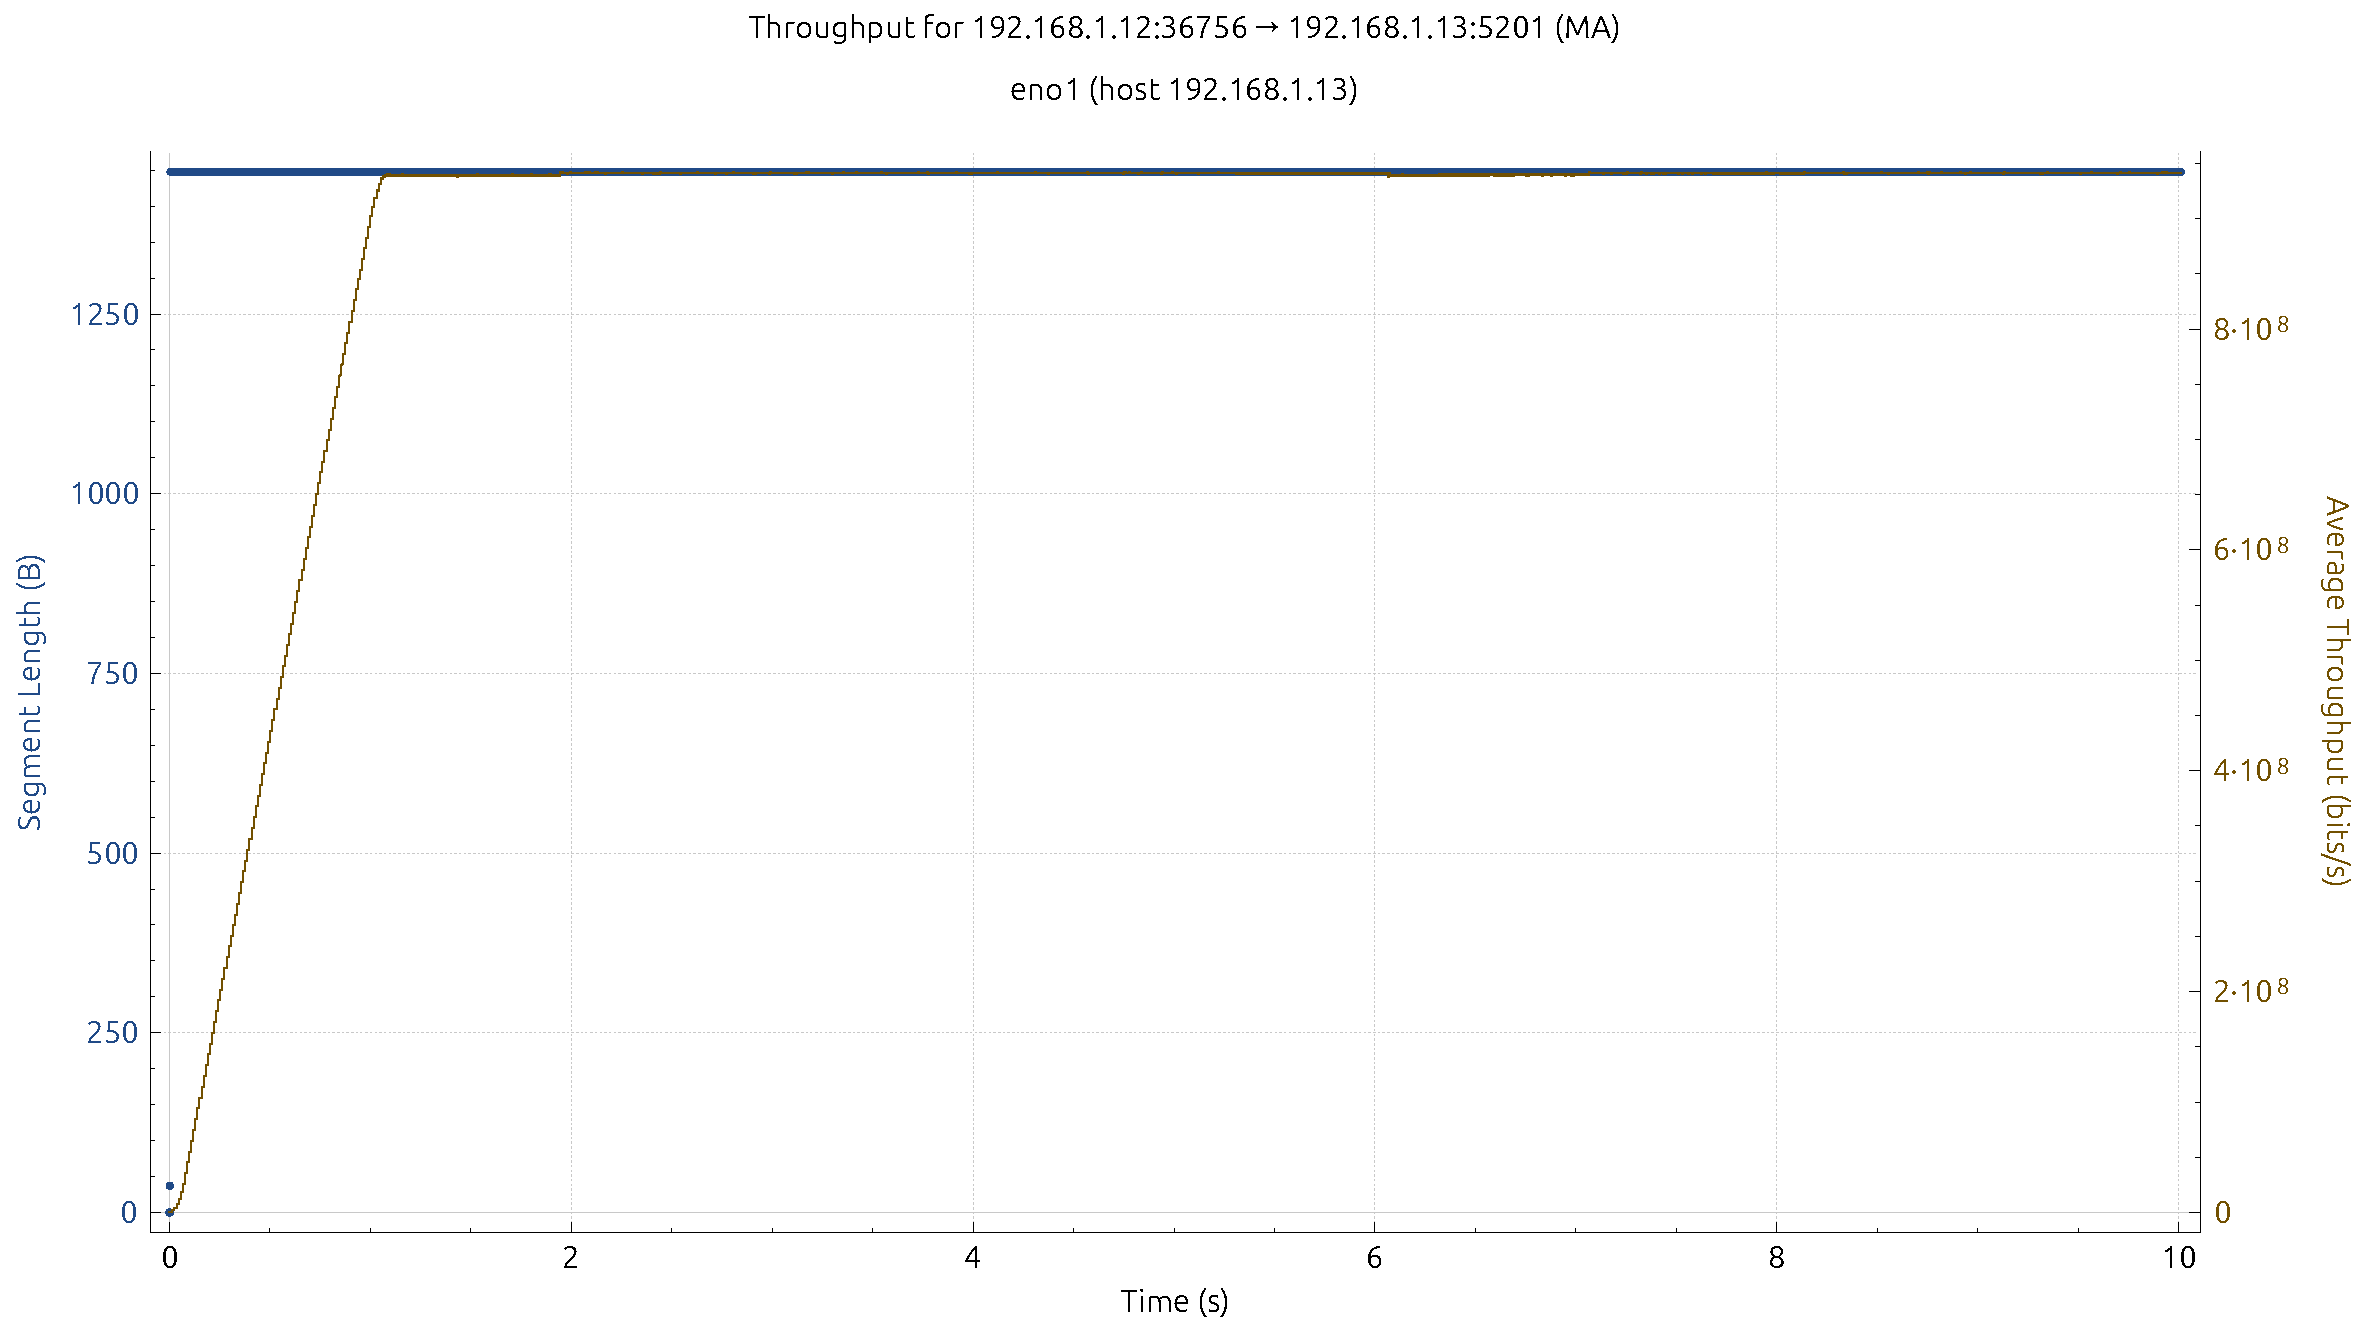
\includegraphics[width=0.9\columnwidth]{images/graphs/Throughput/Throughput_ETH_TCP.pdf}
                    \caption{TCP Throughput in the Ethernet Scenario.}
                    \label{fig:throughput-eth-tcp}
                \end{figure}

                Figure~\ref{fig:rtt-eth-tcp} illustrates the round-trip time (RTT), which remains very low (typically within a few milliseconds), highlighting the minimal latency in wired connections. 
                
                \begin{figure}[ht]
                    \centering
                    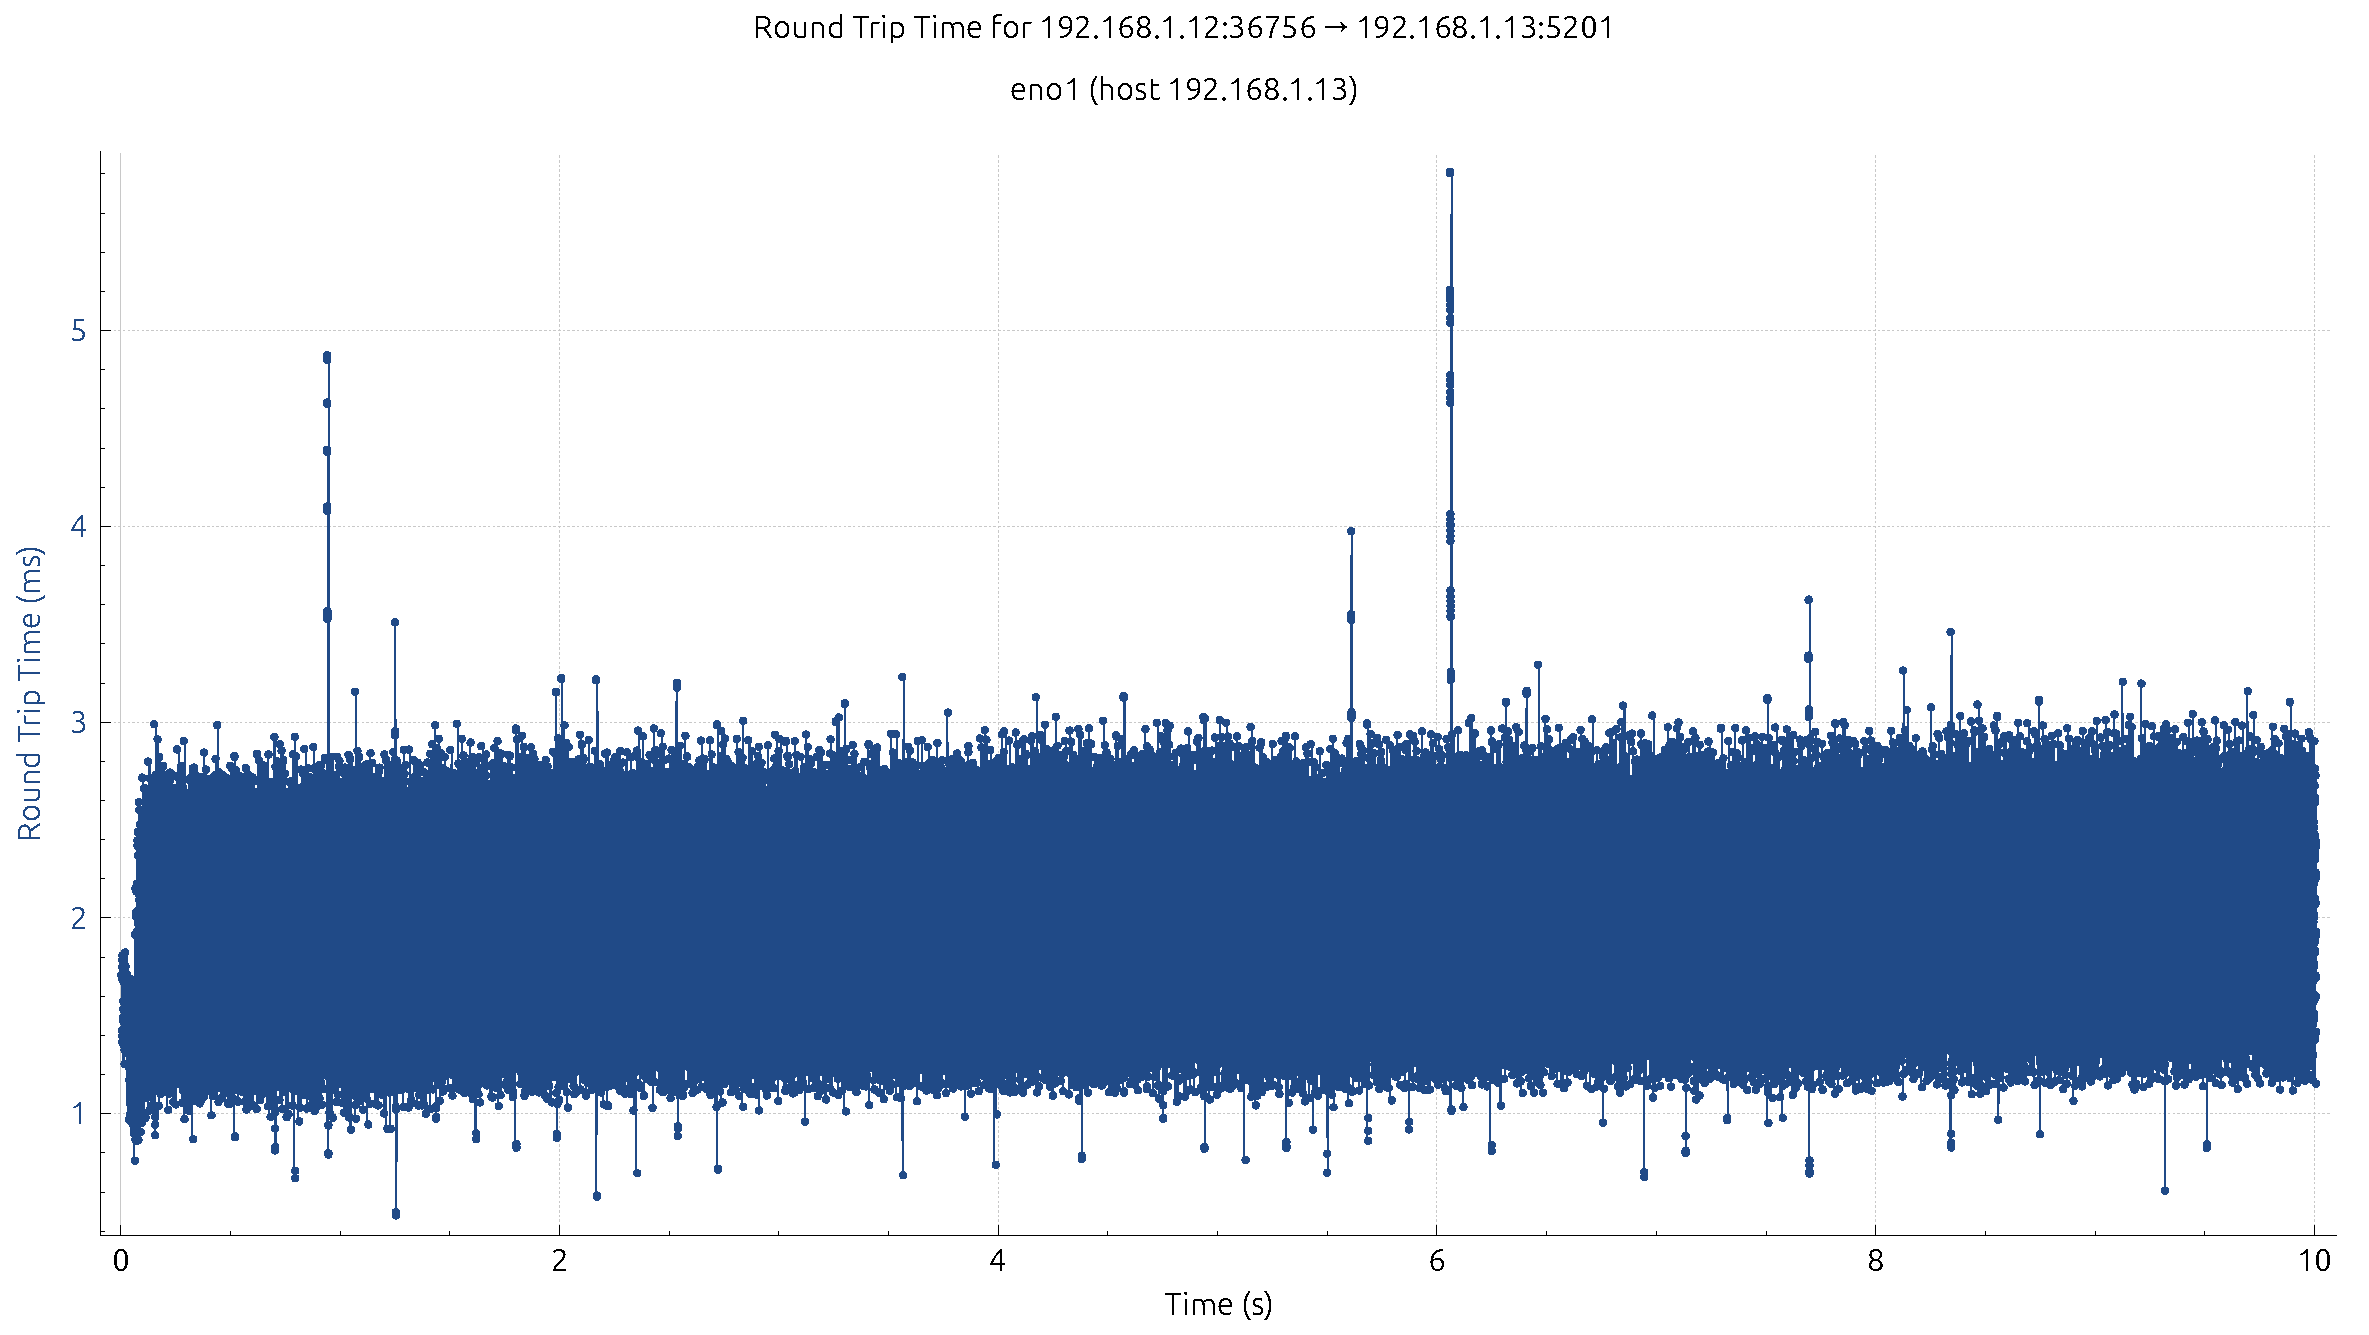
\includegraphics[width=0.9\columnwidth]{images/graphs/RTT/RTT_ETH_TCP.pdf}
                    \caption{TCP Round Trip Time in the Ethernet Scenario.}
                    \label{fig:rtt-eth-tcp}
                \end{figure}

                Furthermore, the I-O graph (Fig.~\ref{fig:io-eth-tcp}) confirms a consistent packet flow with little variation, indicating that the Ethernet setup effectively utilizes the available capacity. 
                
                % \begin{figure}[ht]
                %     \centering
                %     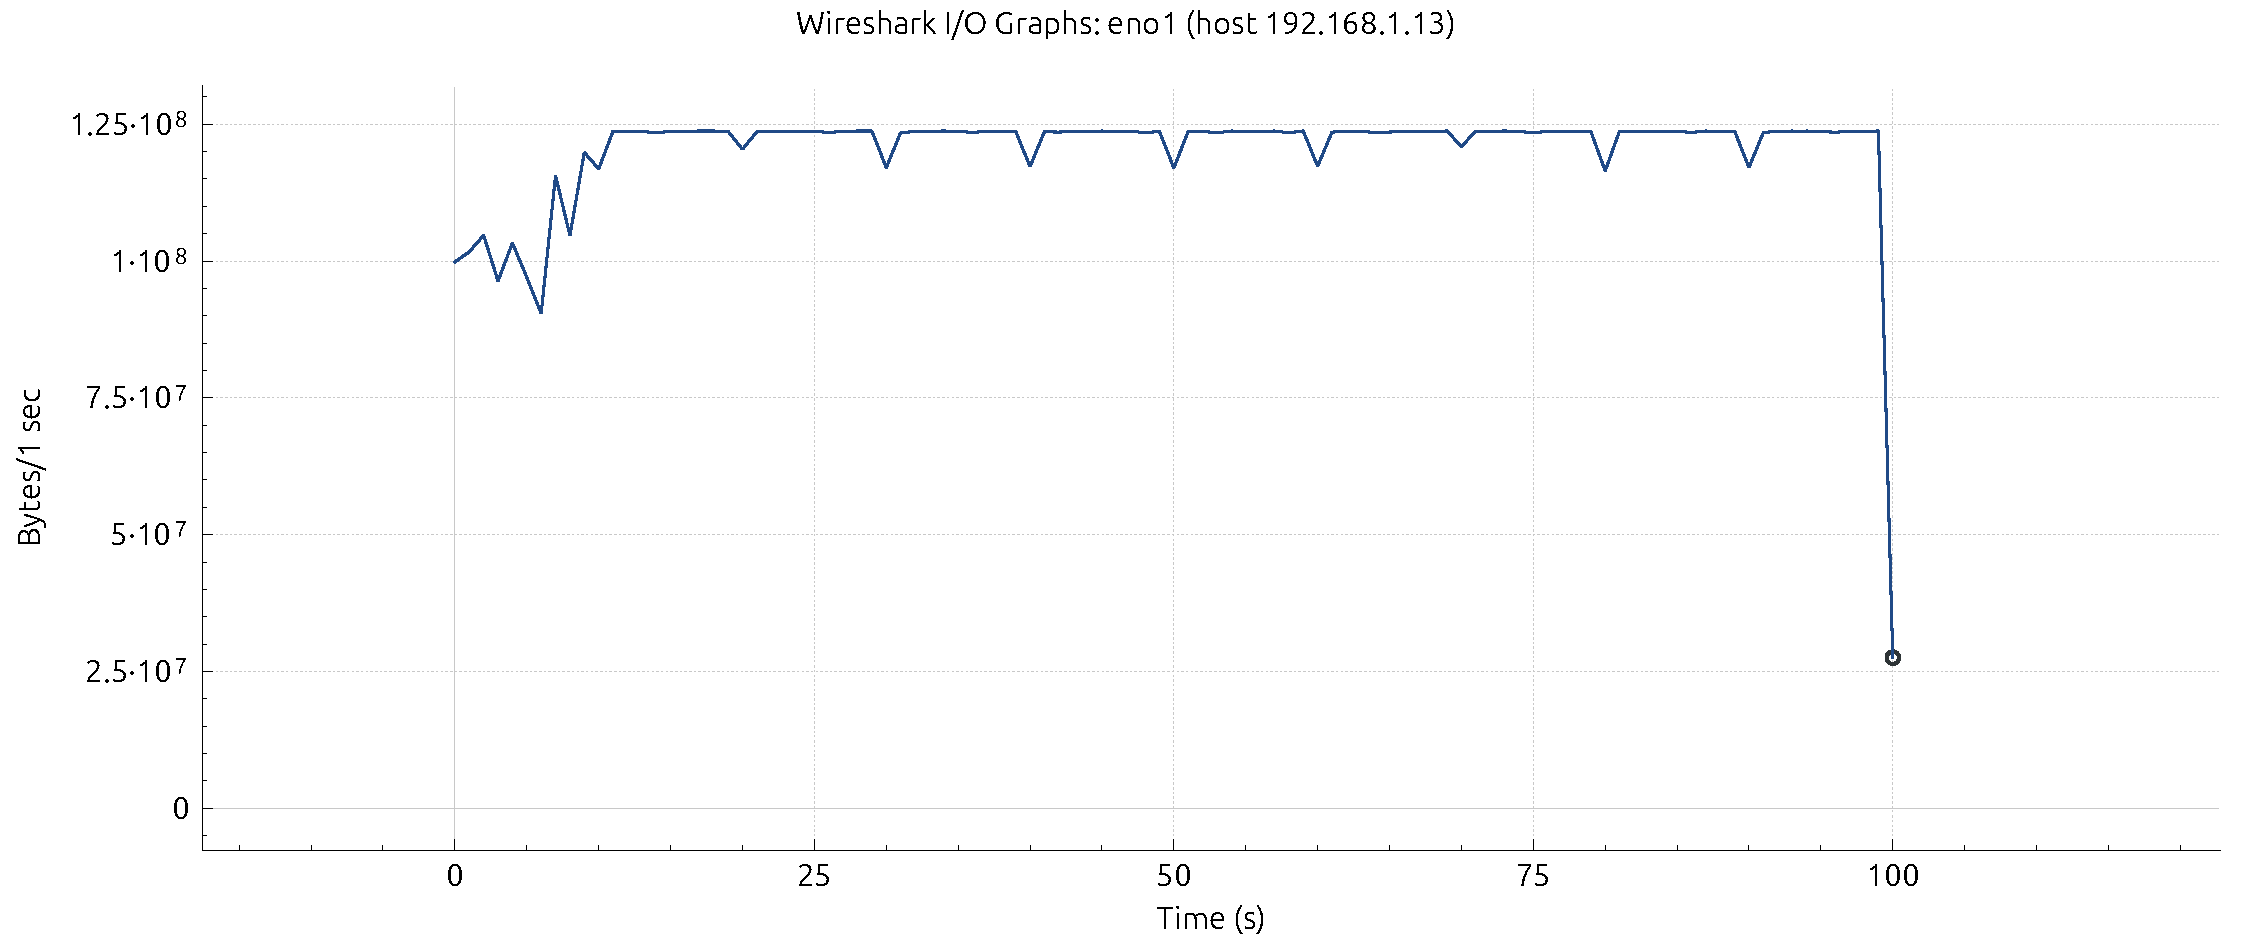
\includegraphics[width=0.9\columnwidth]{images/graphs/I-O/I-O_ETH_TCP.pdf}
                %     \caption{Wireshark I-O Graph for TCP in the Ethernet Scenario.}
                %     \label{fig:io-eth-tcp}
                % \end{figure}

                Overall, the Ethernet scenario demonstrates a near-ideal performance with high throughput and minimal latency, closely matching the theoretical predictions.

            \item \textbf{Both WiFi:} \\
                In the WiFi scenario, the throughput graph (Fig.~\ref{fig:throughput-wifi-tcp}) shows an initial ramp-up phase during the first 2 seconds, after which the throughput fluctuates around an average value that is significantly lower than the theoretical maximum of approximately 347\,Mbps. 
                These fluctuations suggest that protocol overhead, wireless interference, and the half-duplex nature of WiFi adversely affect performance. \\
                
                \begin{figure}[ht]
                    \centering
                    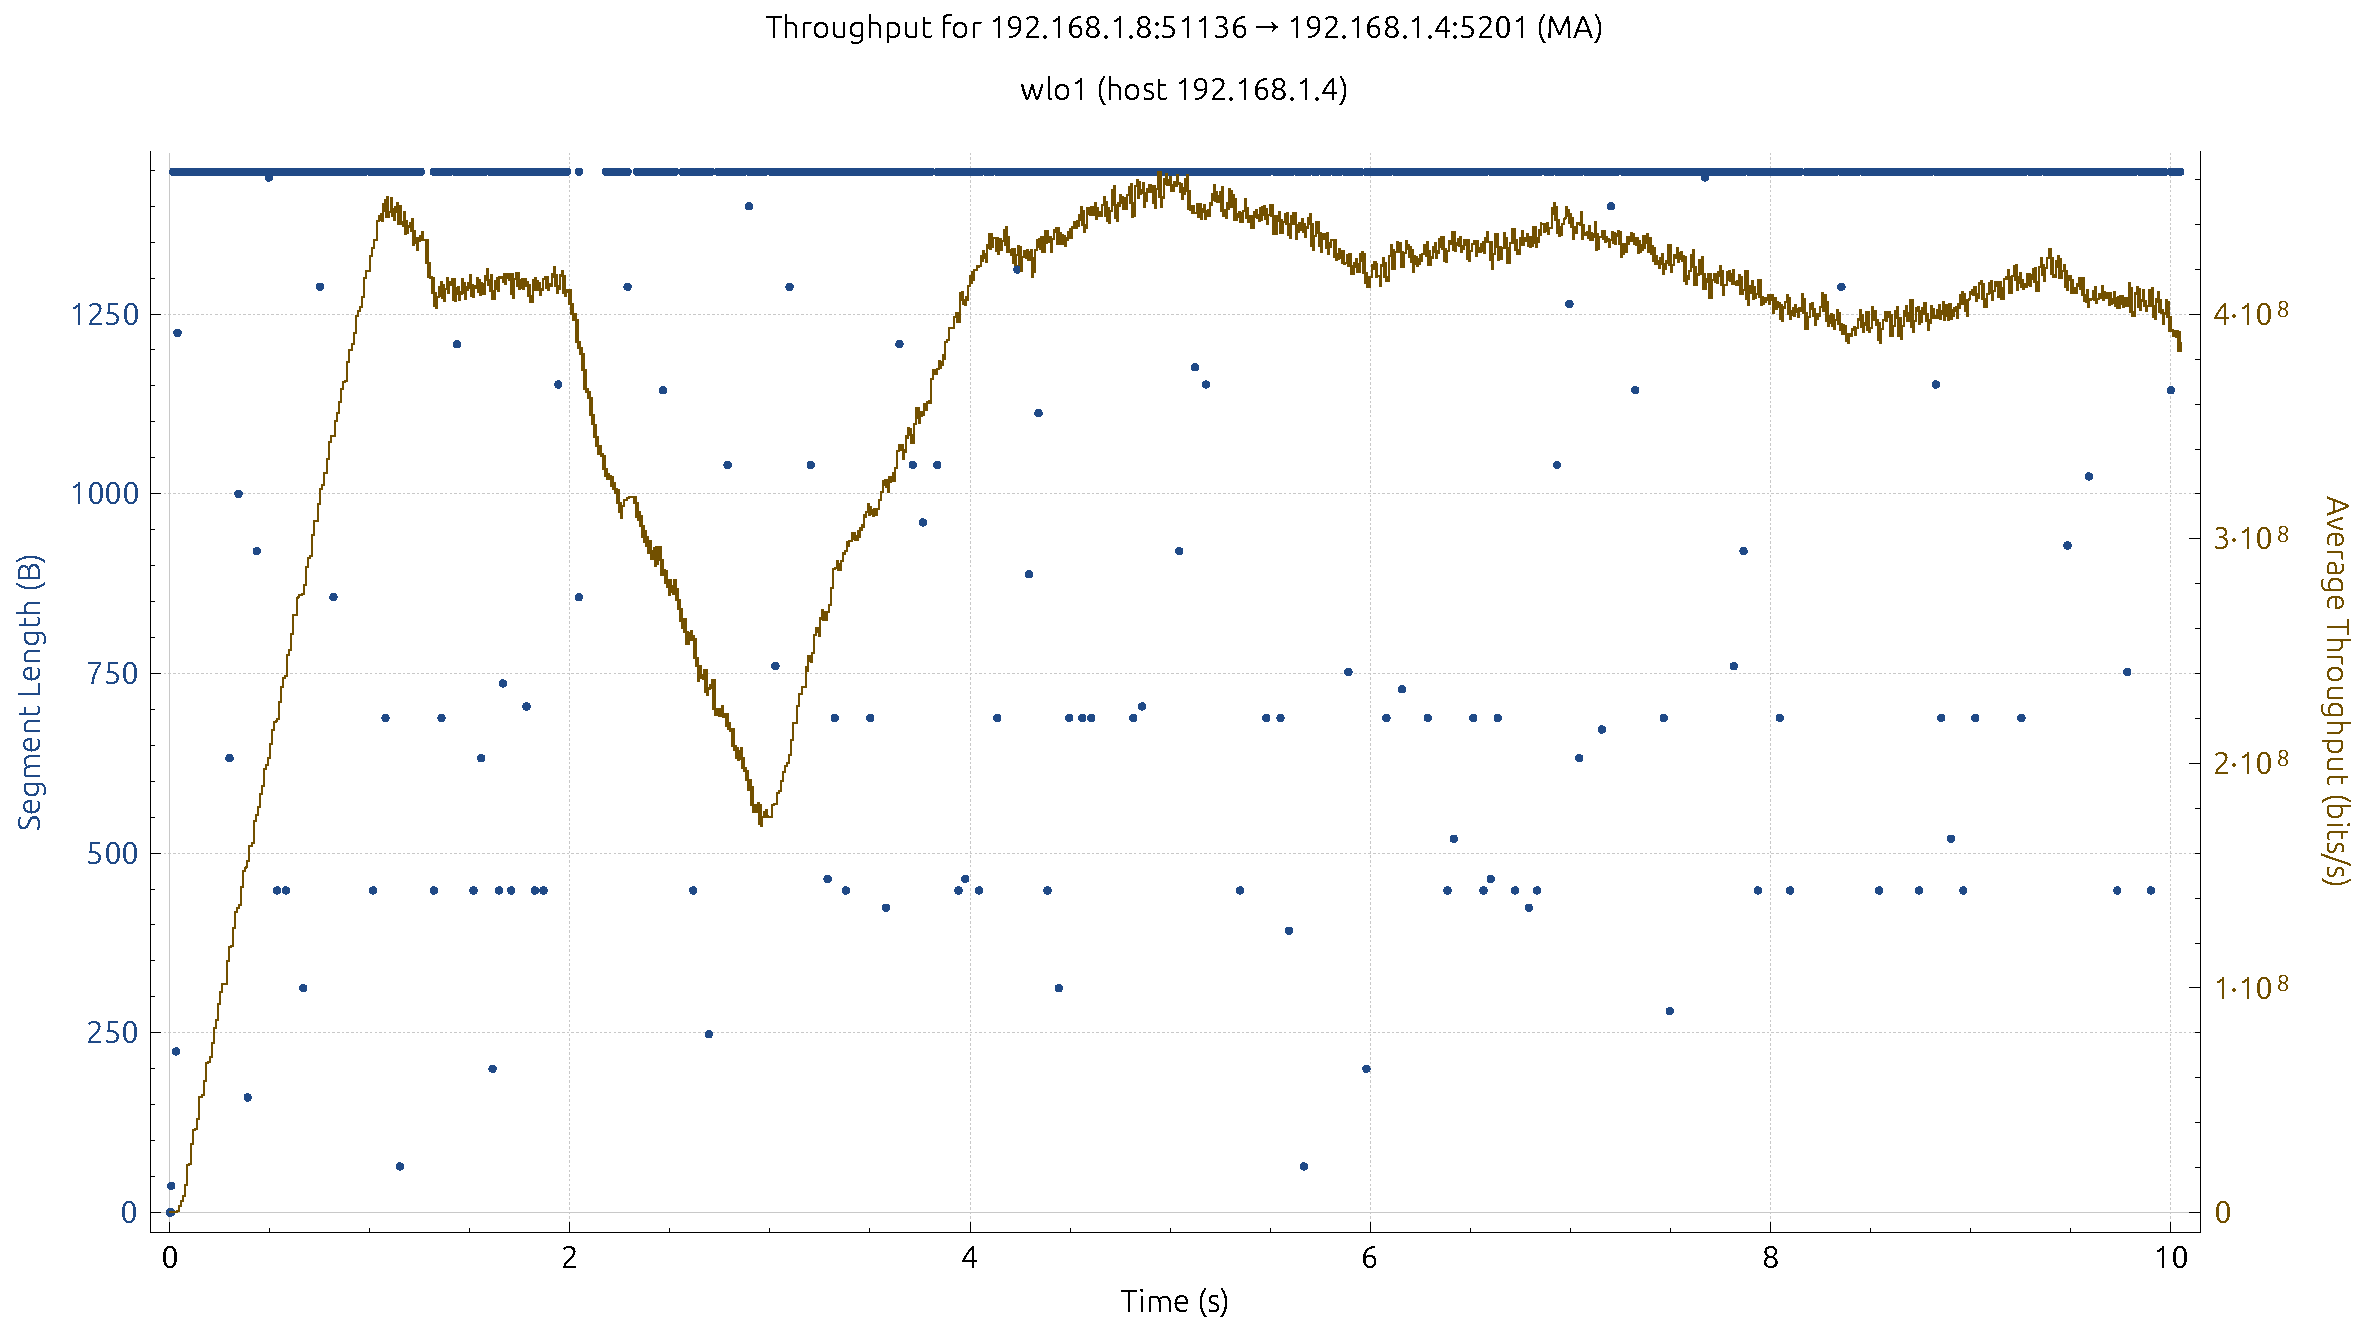
\includegraphics[width=0.9\columnwidth]{images/graphs/Throughput/Throughput_WiFi_TCP.pdf}
                    \caption{TCP Throughput in the WiFi Scenario.}
                    \label{fig:throughput-wifi-tcp}
                \end{figure}

                The round-trip time (RTT) measurements (Fig.~\ref{fig:rtt-wifi-tcp}) reveal RTT values ranging from about 50 to 200\,ms, indicating intermittent delays likely due to congestion and contention in the wireless medium. \\
                
                \begin{figure}[ht]
                    \centering
                    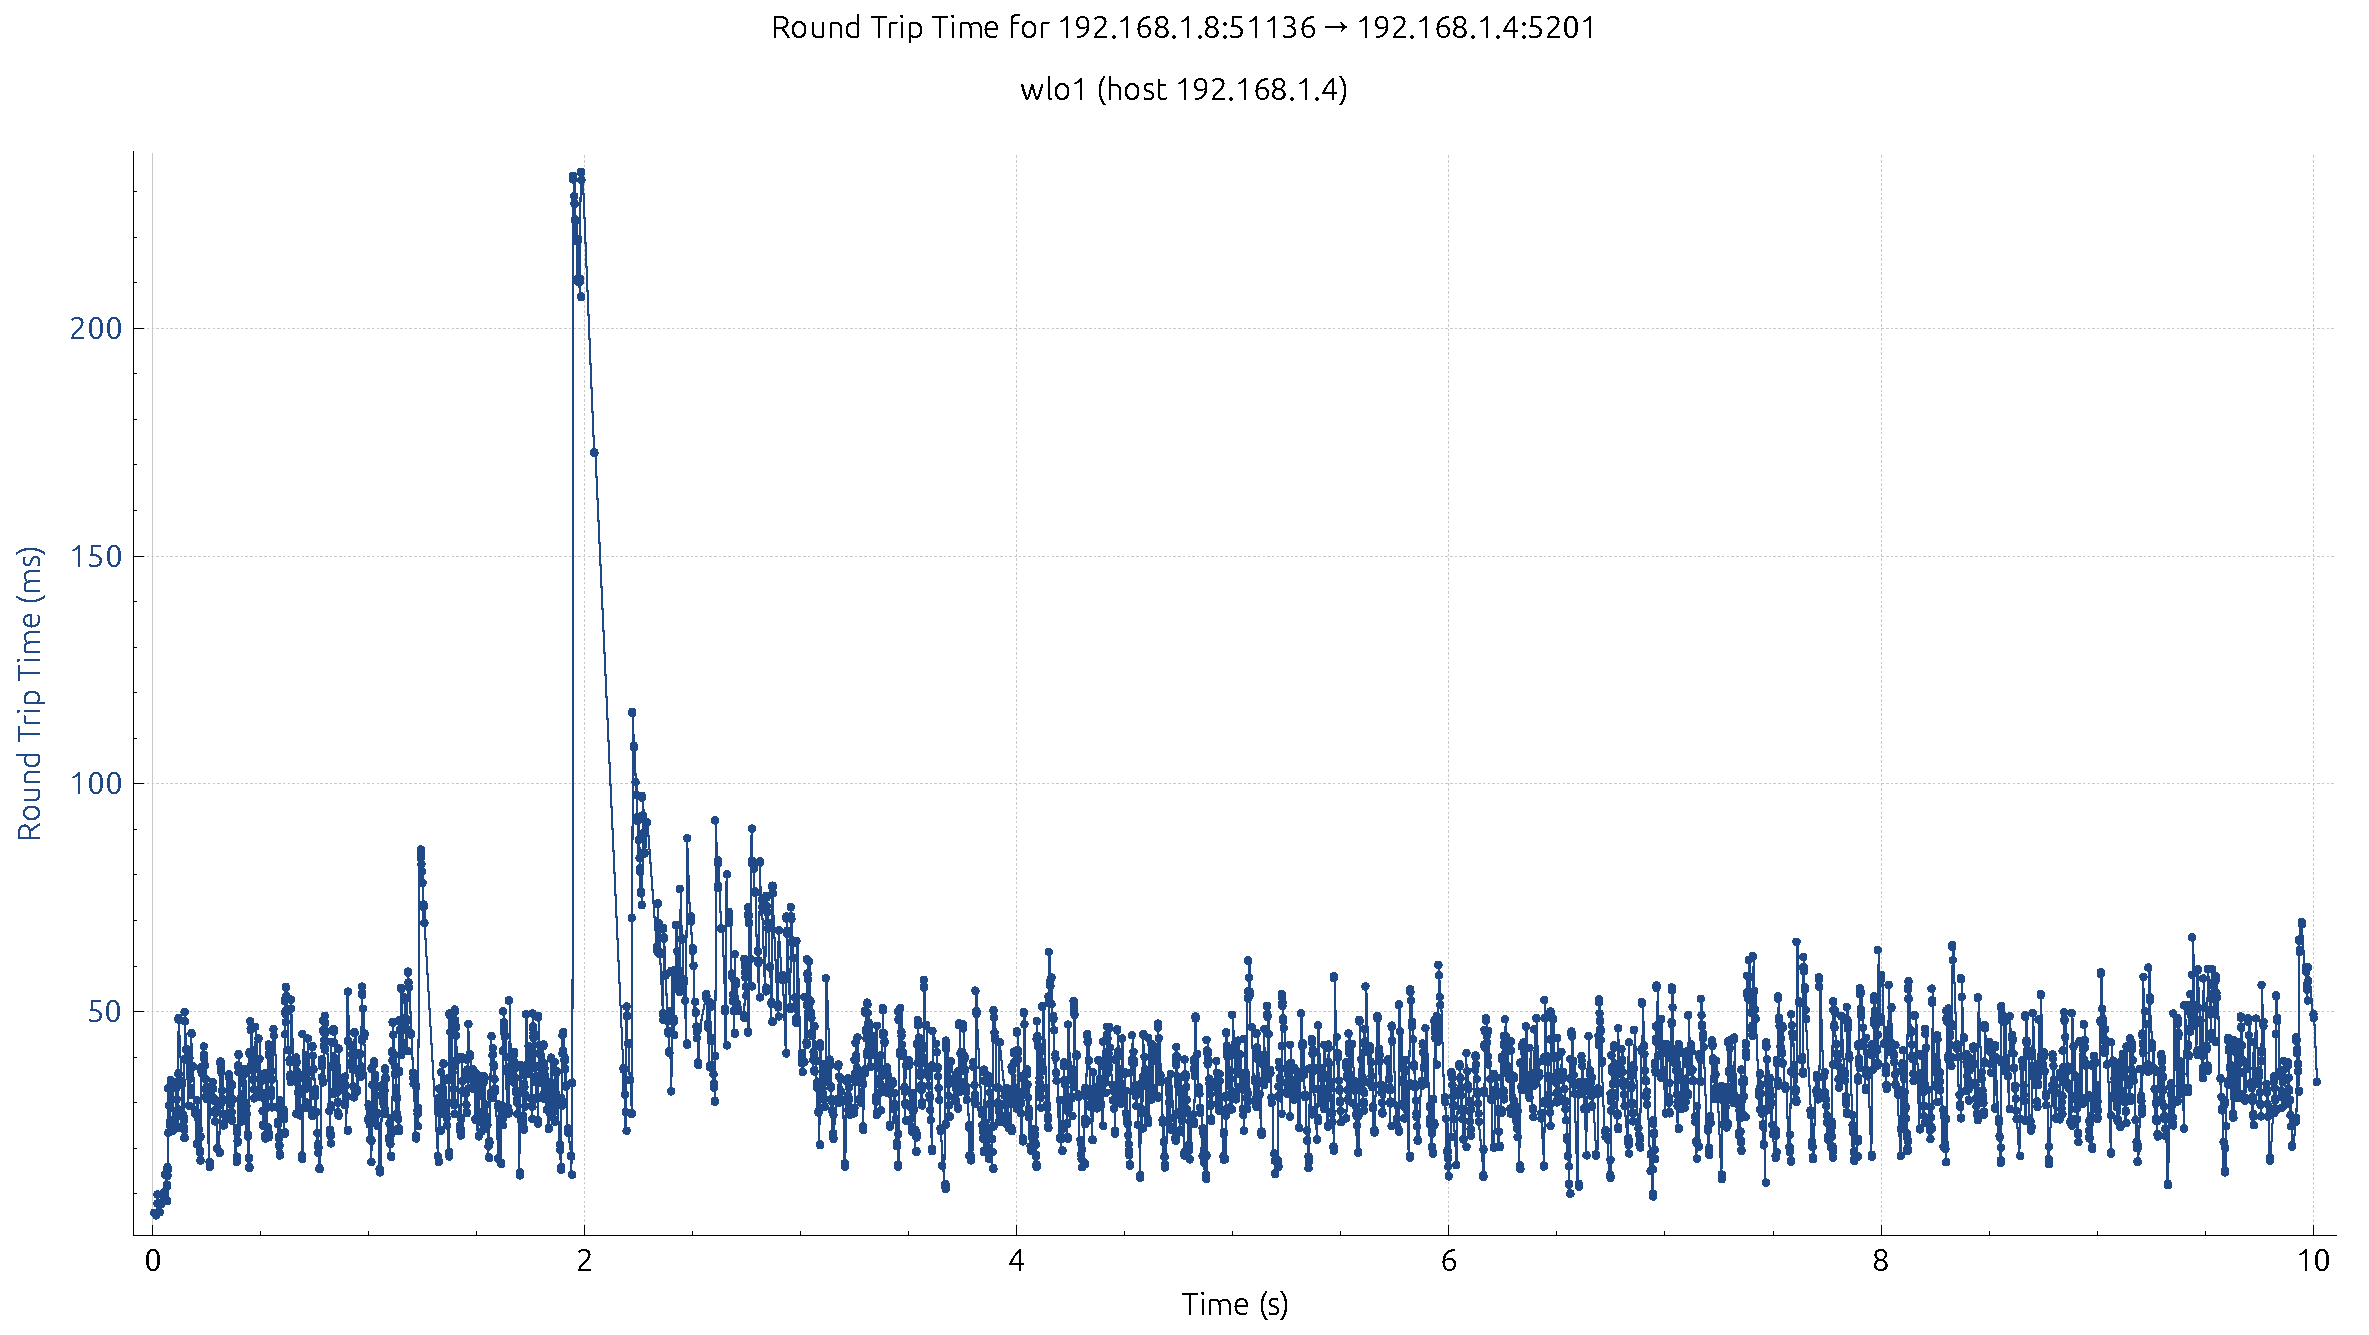
\includegraphics[width=0.9\columnwidth]{images/graphs/RTT/RTT_WiFi_TCP.pdf}
                    \caption{TCP Round Trip Time in the WiFi Scenario.}
                    \label{fig:rtt-wifi-tcp}
                \end{figure}    

                Furthermore, the I-O graph (Fig.~\ref{fig:io-wifi-tcp}) illustrates a variable number of transmitted packets per interval, reflecting the dynamic nature of WiFi communication where channel conditions and collision avoidance mechanisms influence performance.
                
                % \begin{figure}[ht]
                %     \centering
                %     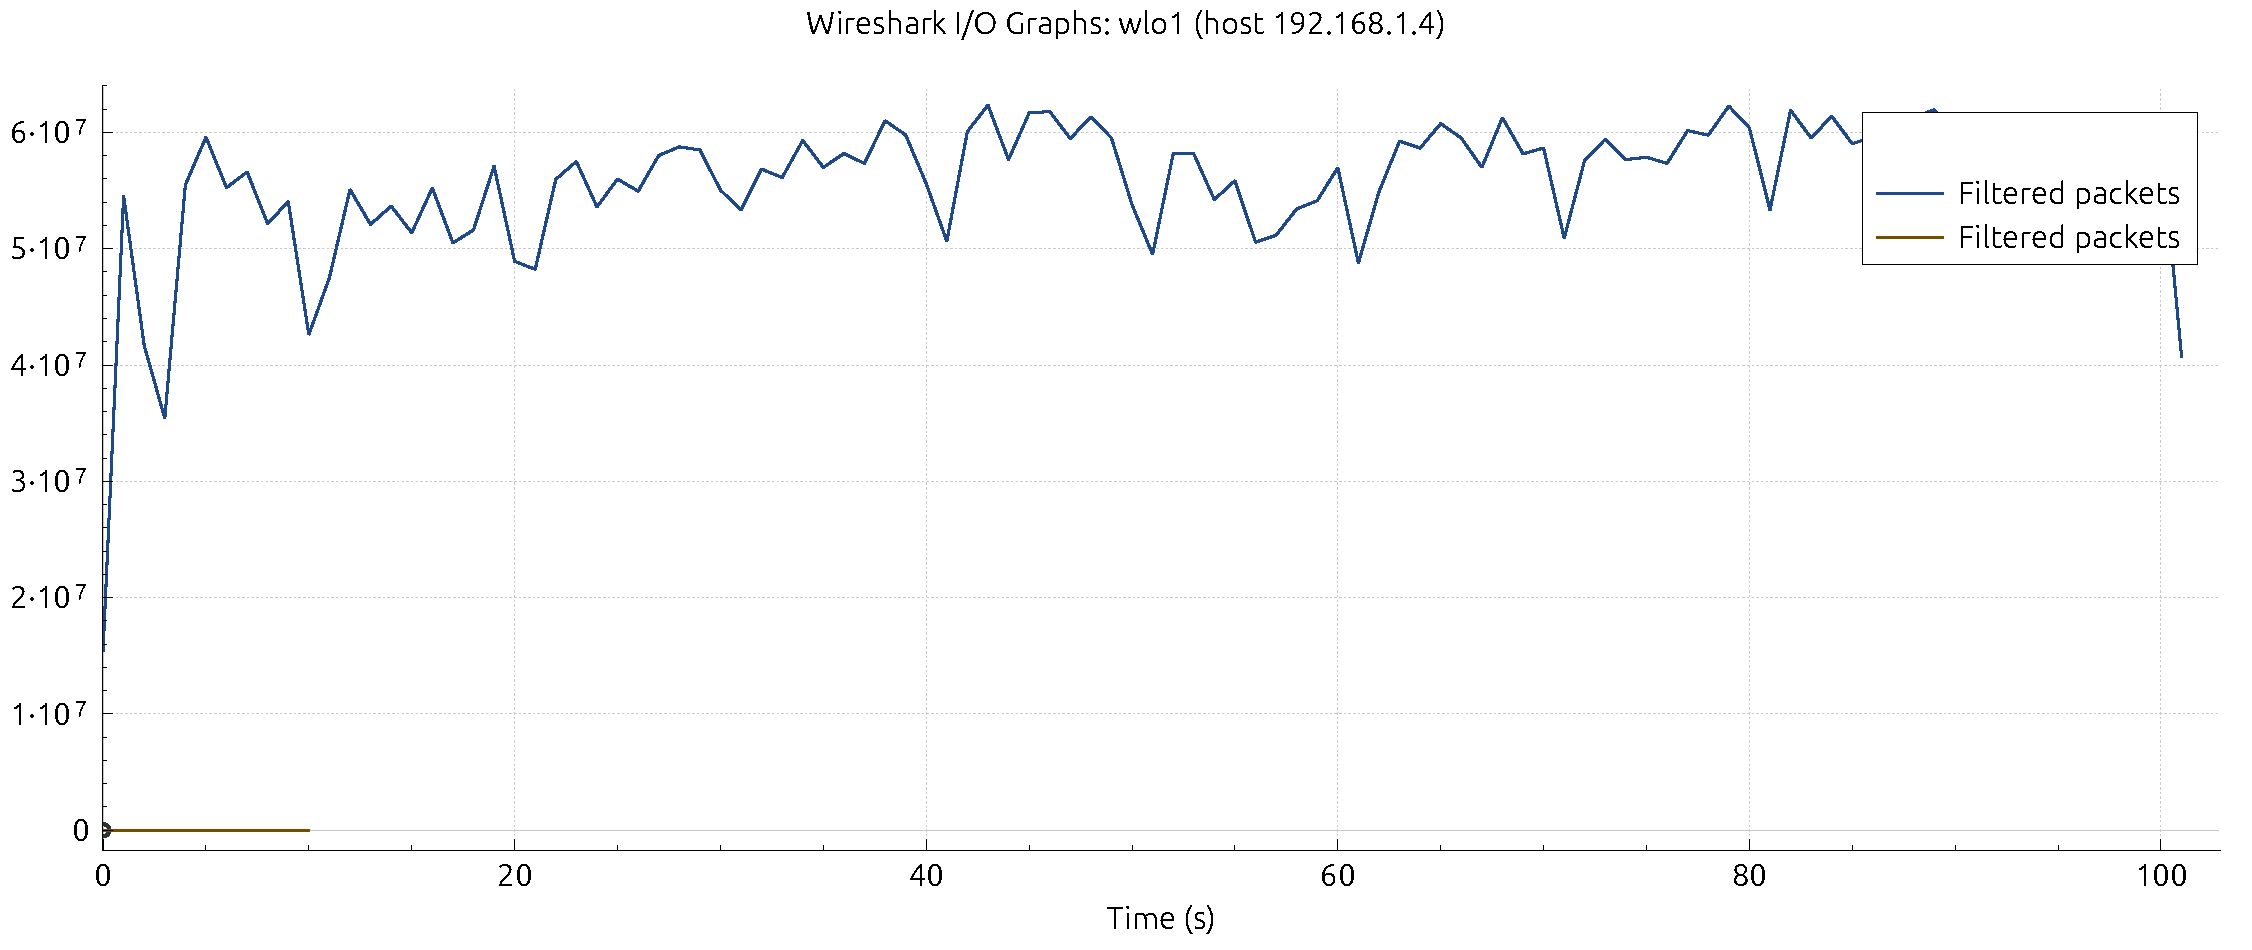
\includegraphics[width=0.9\columnwidth]{images/graphs/I-O/I-O_WiFi_TCP.pdf}
                %     \caption{Wireshark I-O Graph for TCP in the WiFi Scenario.}
                %     \label{fig:io-wifi-tcp}
                % \end{figure}

                Overall, while the theoretical capacity for TCP over WiFi is estimated to be around 347\,Mbps, the experimental data indicate that real-world factors substantially reduce the effective throughput.

            \item \textbf{Mixed:} \\
                Figure~\ref{fig:throughput-mix-tcp} displays the TCP throughput for the mixed configuration. 
                The graph shows that the throughput reaches a stable level after an initial ramp-up phase, although it remains below the Ethernet scenario and is consistent with the expected reduction due to the reliance on the wireless link. \\

                \begin{figure}[ht]
                    \centering
                    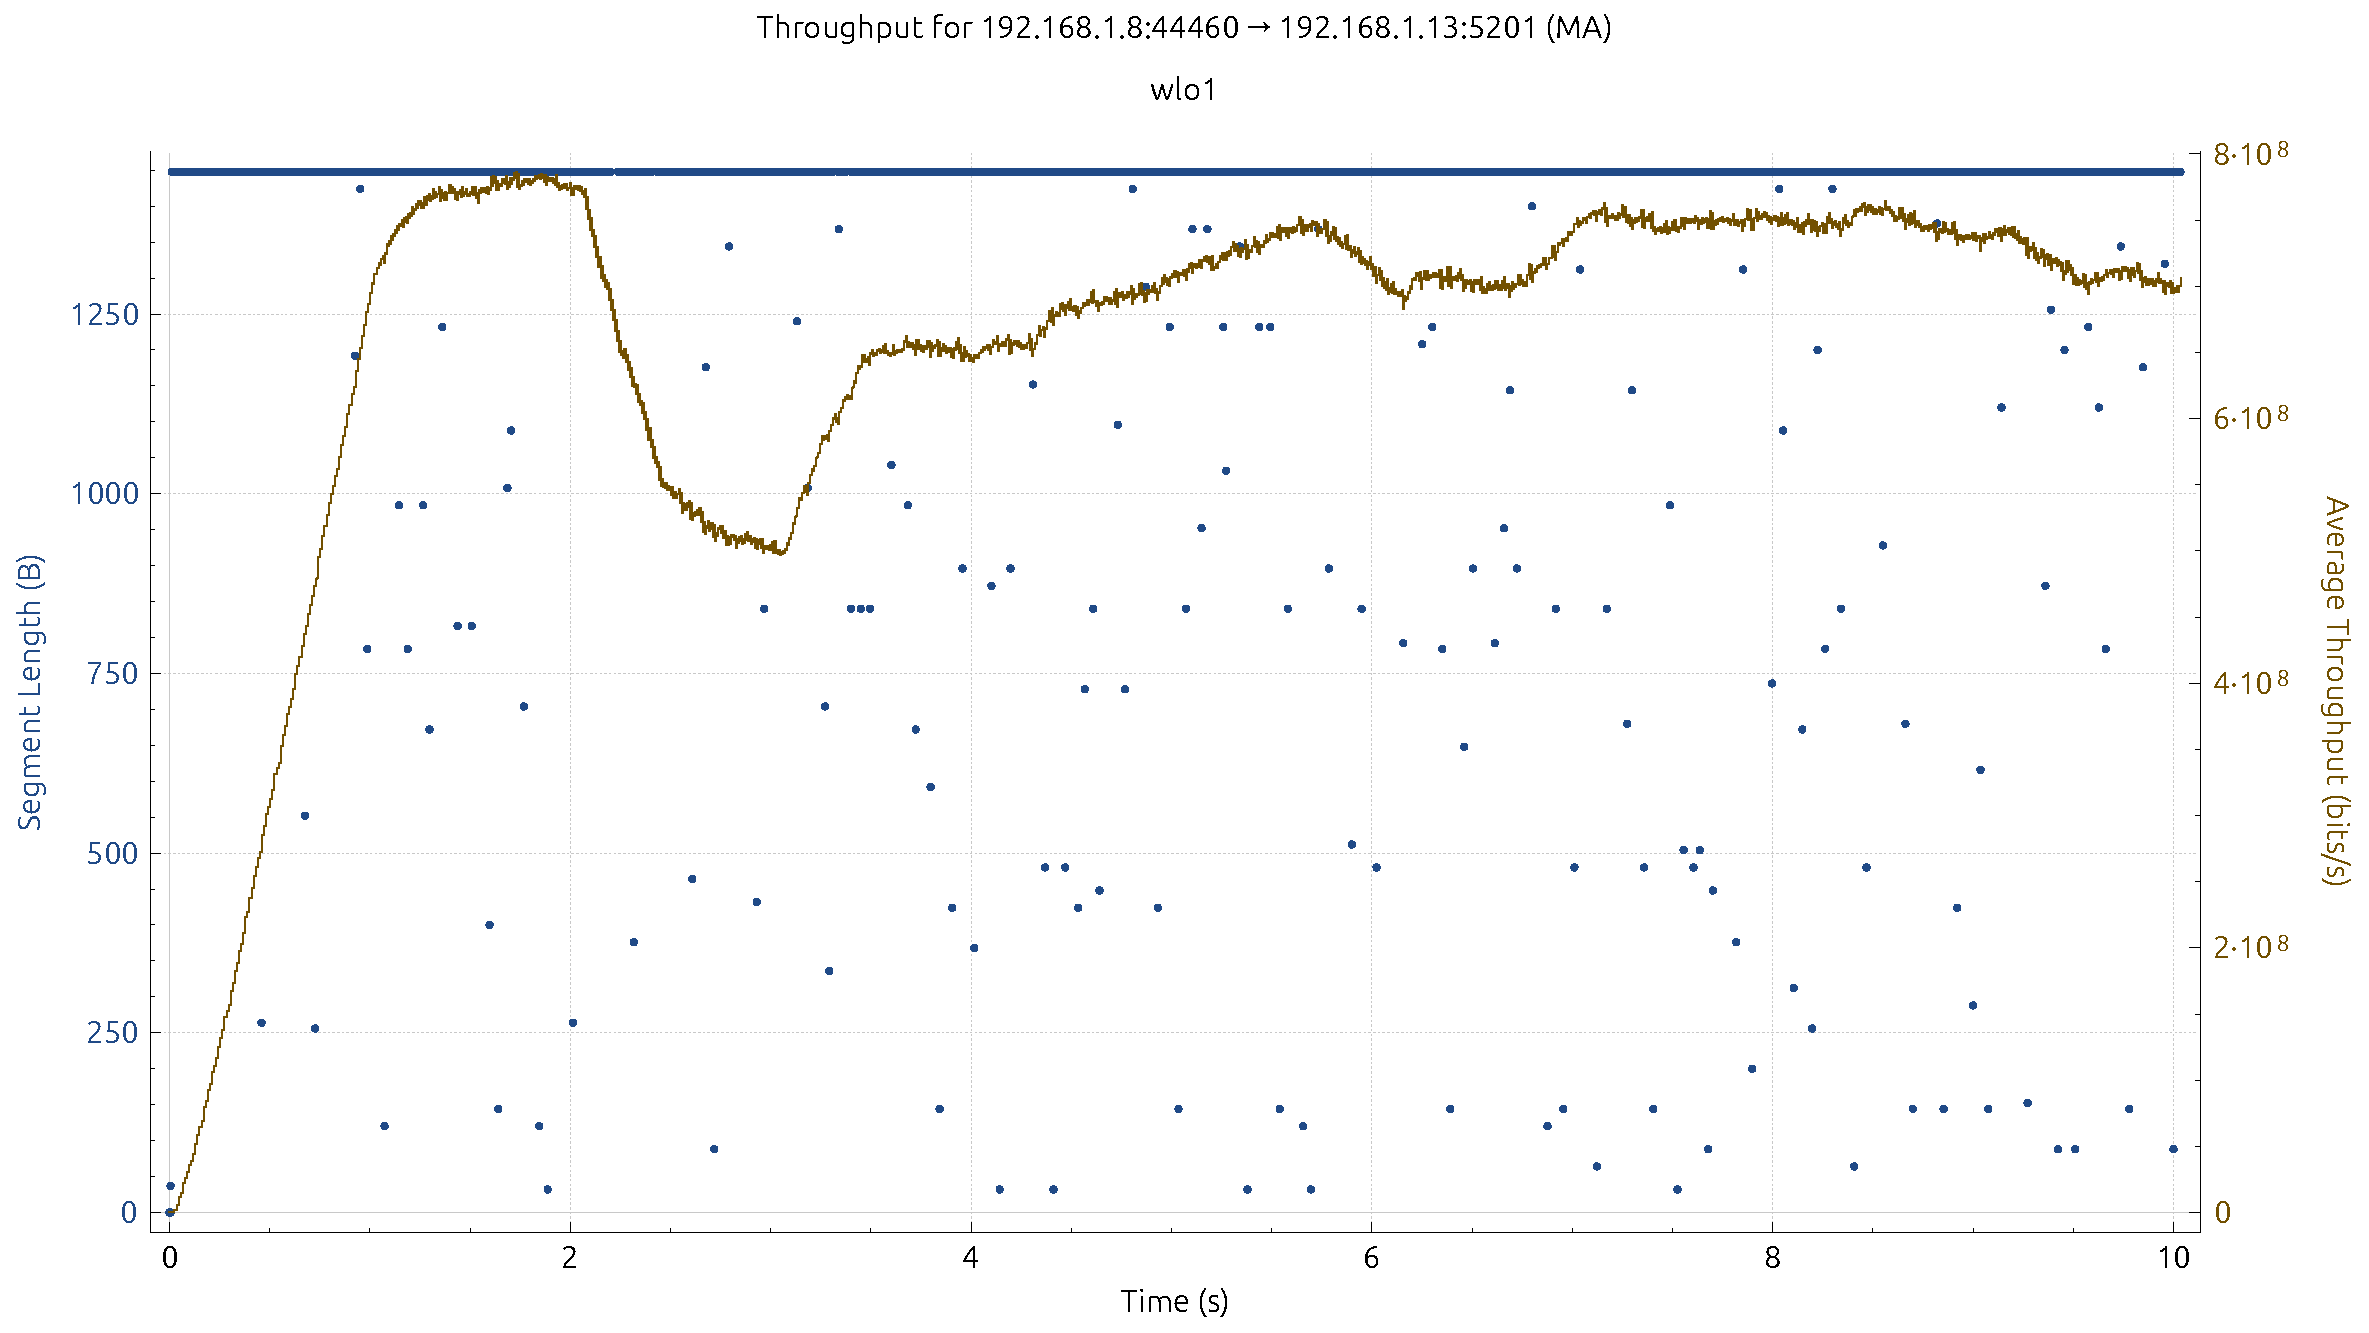
\includegraphics[width=0.9\columnwidth]{images/graphs/Throughput/Throughput_MIX_TCP.pdf}
                    \caption{TCP Throughput in the Mixed Ethernet/WiFi Scenario.}
                    \label{fig:throughput-mix-tcp}
                \end{figure}

                The round-trip time (RTT) measurements, presented in Figure~\ref{fig:rtt-mix-tcp}, indicate moderate latency, with RTT values generally remaining within a lower range compared to the pure WiFi scenario. 
                This suggests that the wired segment helps in reducing overall latency. \\

                \begin{figure}[ht]
                    \centering
                    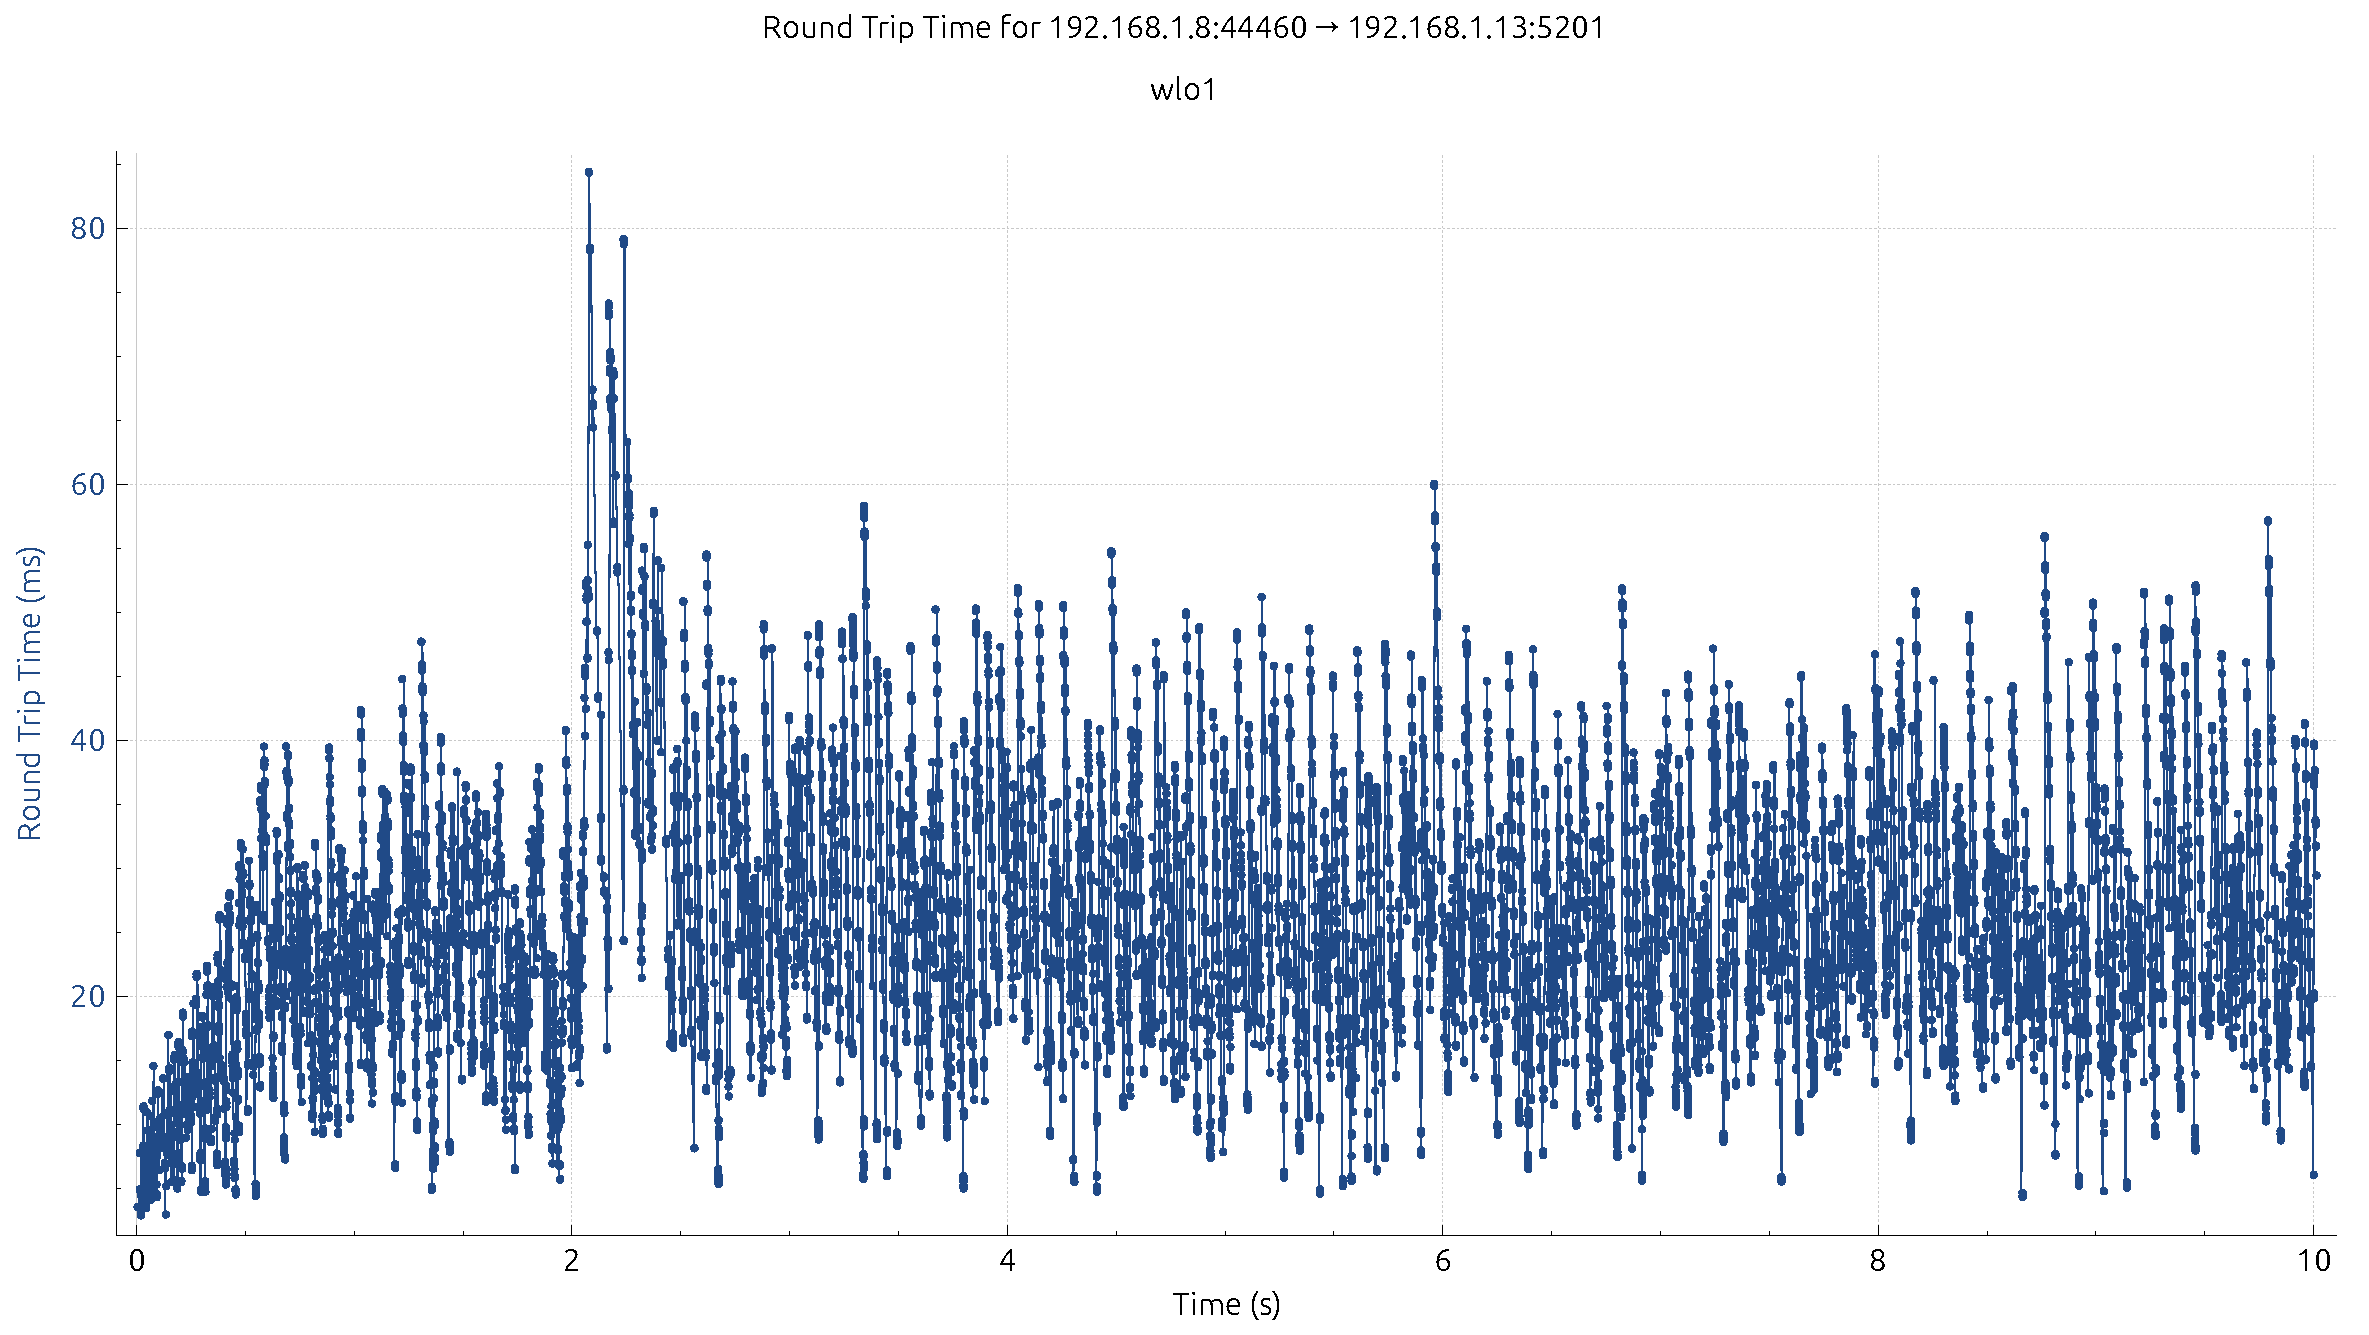
\includegraphics[width=0.9\columnwidth]{images/graphs/RTT/RTT_MIX_TCP.pdf}
                    \caption{TCP Round Trip Time in the Mixed Ethernet/WiFi Scenario.}
                    \label{fig:rtt-mix-tcp}
                \end{figure}

                The I-O graph for TCP (Fig.~\ref{fig:io-mix-tcp}) shows a relatively steady packet flow over the test intervals, confirming that the mixed configuration maintains a stable performance despite the inherent variability of the wireless link.

                % \begin{figure}[ht]
                %     \centering
                %     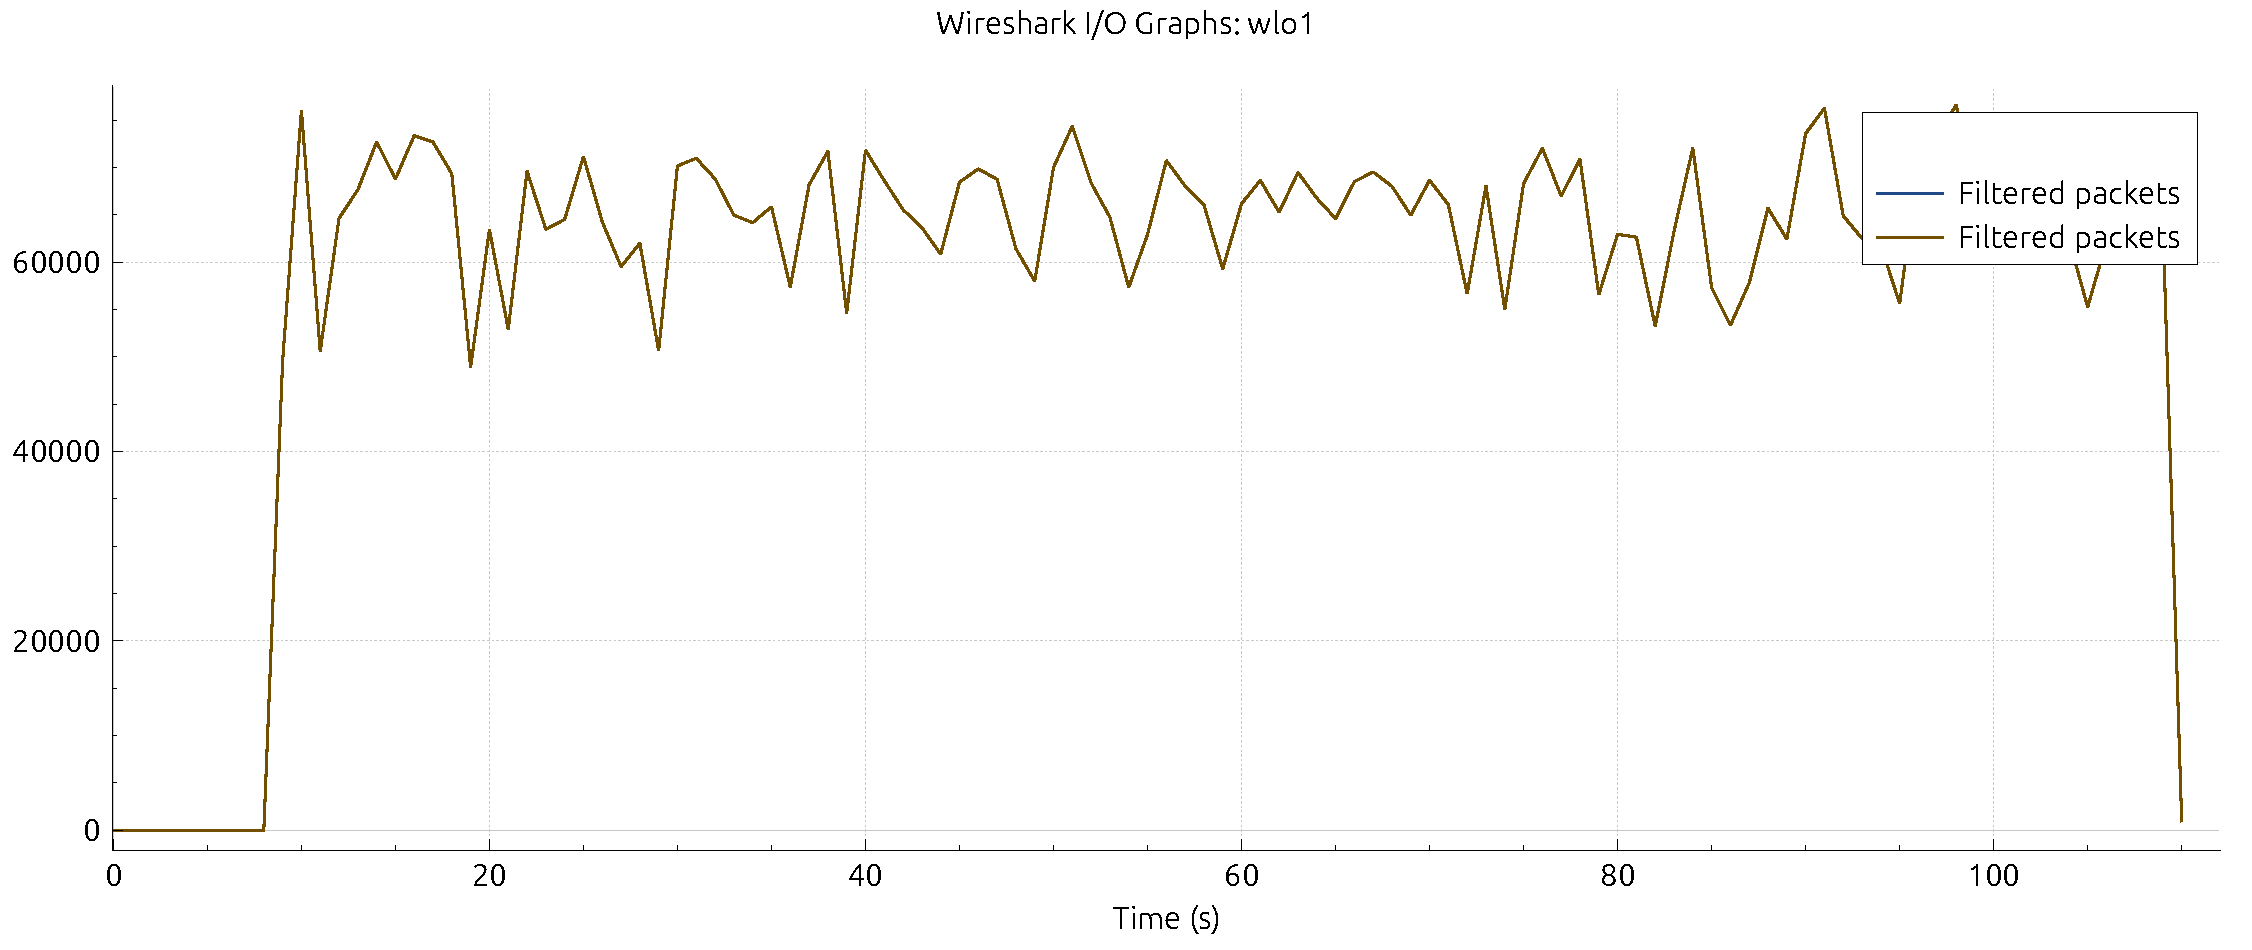
\includegraphics[width=0.9\columnwidth]{images/graphs/I-O/I-O_MIX_TCP.pdf}
                %     \caption{Wireshark I-O Graph for TCP in the Mixed Scenario.}
                %     \label{fig:io-mix-tcp}
                % \end{figure}
                
            \item[3a.] \textbf{Shared Capacity:} \\
                In this scenario, a third host connected to the same access point was concurrently downloading the film "Natale a Rio" (directed by Neri Parenti), which introduced significant interference during the tests. 
                This additional traffic compromised the available network capacity, leading to degraded performance.
                Figure~\ref{fig:throughput-mitm-tcp} shows the TCP throughput under this shared capacity condition. 
                Compared to the mixed scenario without interference, the throughput exhibits a notable decrease. 
                The average throughput is lower, reflecting the reduced available bandwidth caused by the competing download traffic.

                \begin{figure}[ht]
                    \centering
                    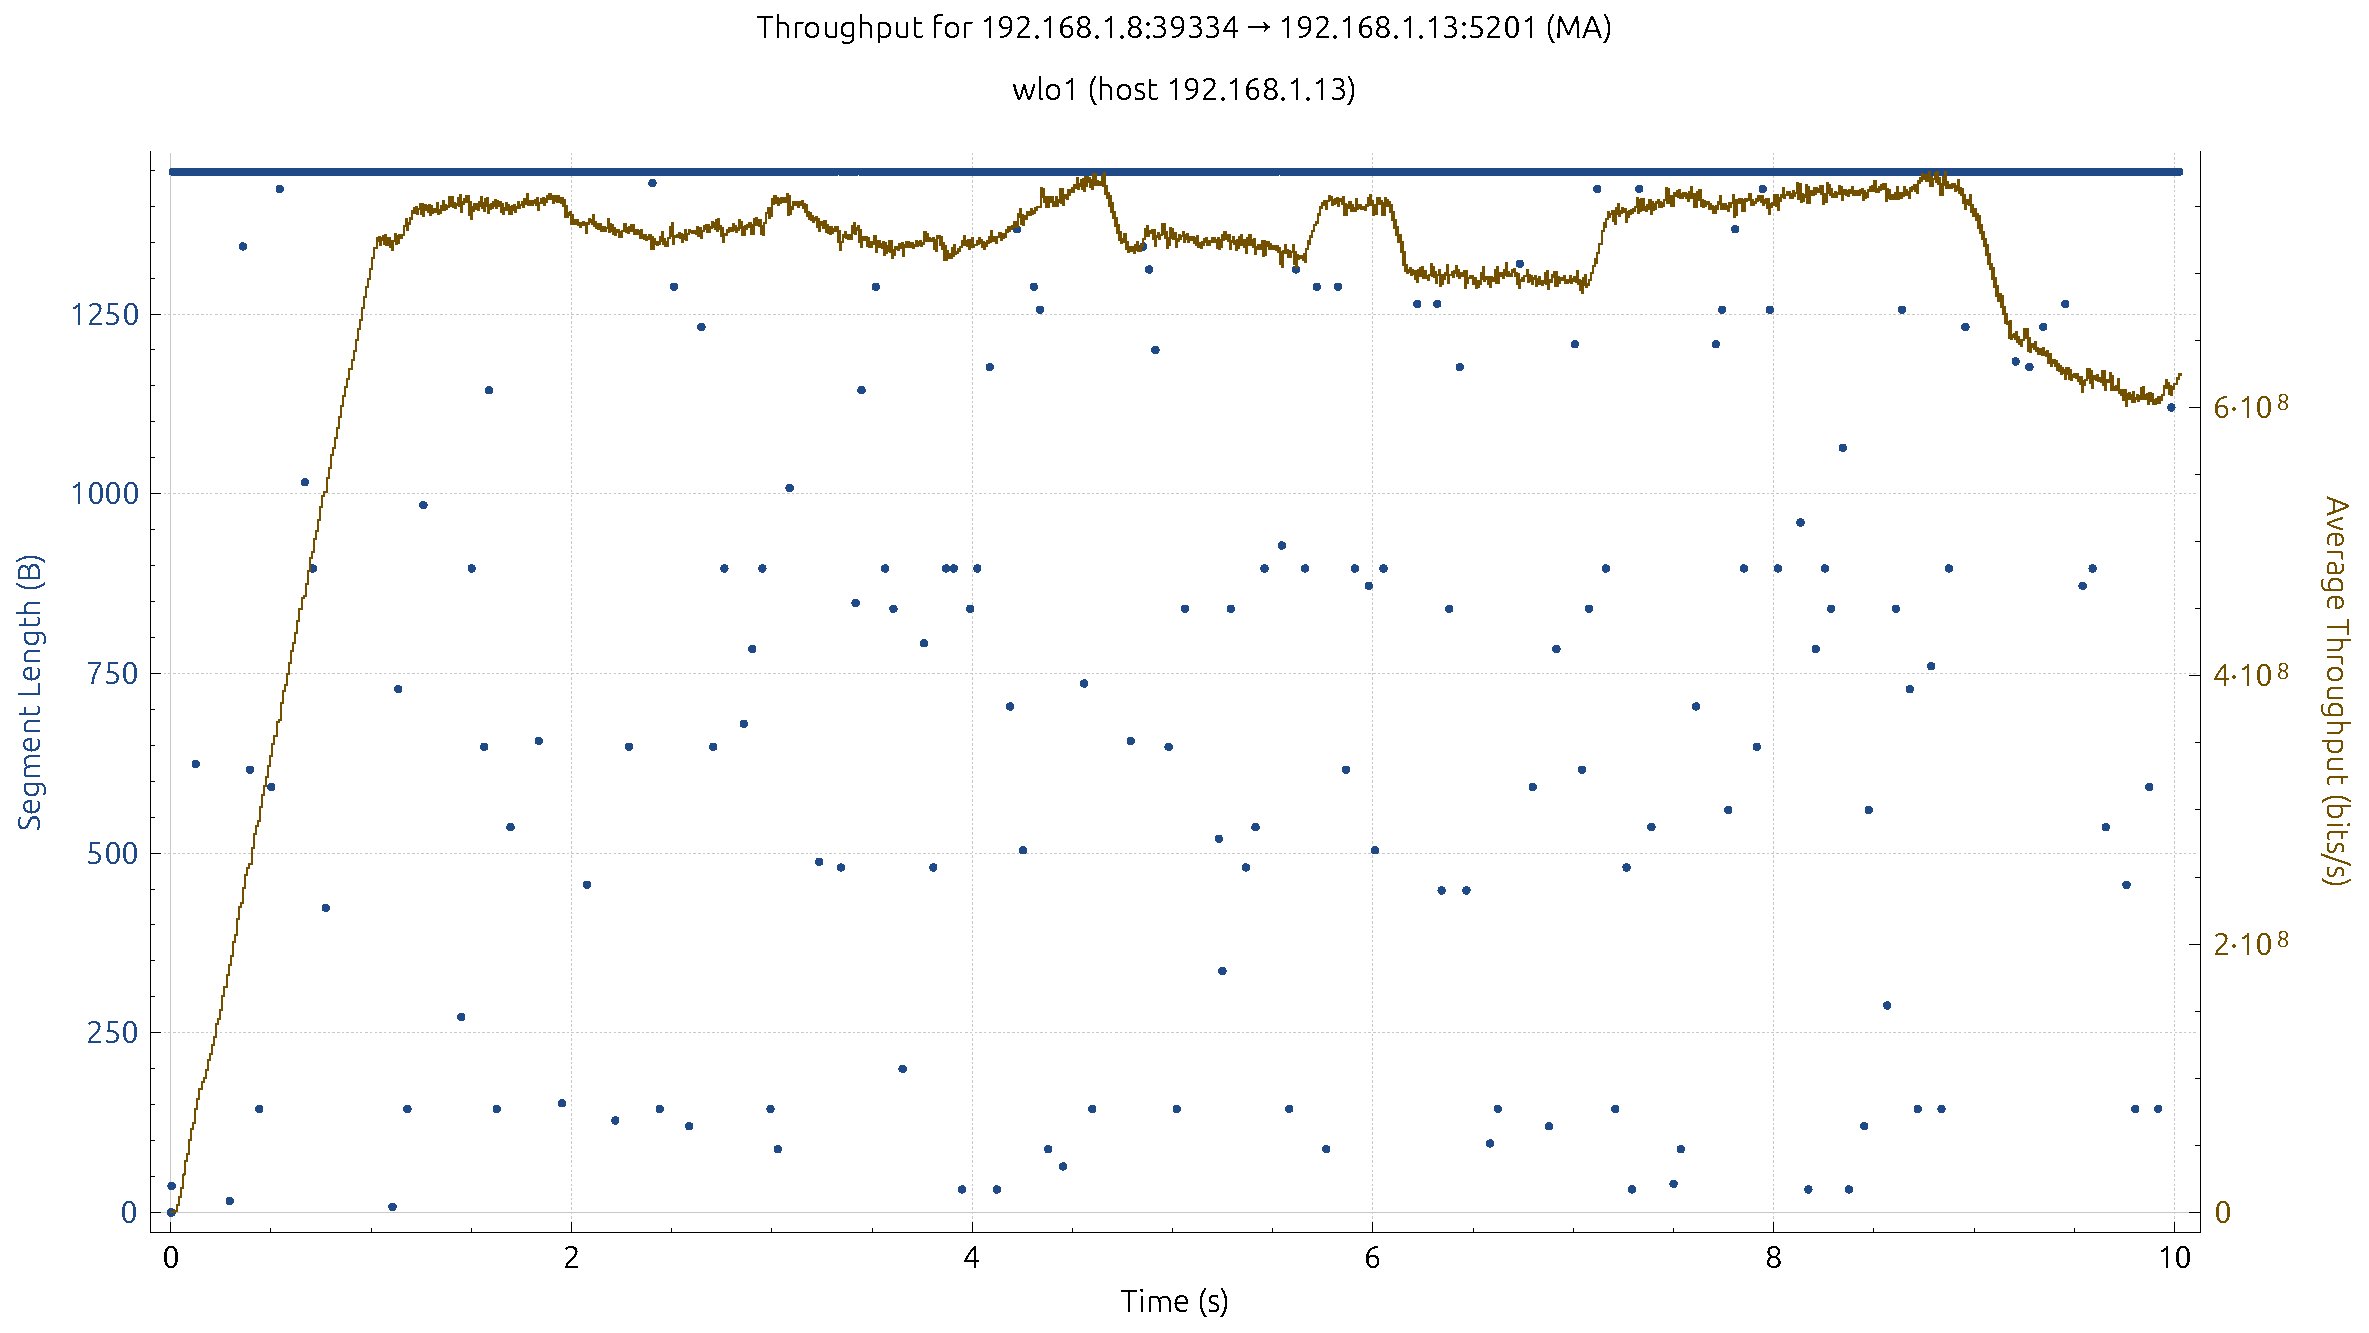
\includegraphics[width=0.9\columnwidth]{images/graphs/Throughput/Throughput_MIX_MITM_TCP.pdf}
                    \caption{TCP Throughput in the Shared Capacity Scenario (with third-host interference).}
                    \label{fig:throughput-mitm-tcp}
                \end{figure}

                The round-trip time measurements (Fig.~\ref{fig:rtt-mitm-tcp}) indicate increased variability and slightly elevated latency. 
                Although the RTT values remain relatively moderate, the fluctuations suggest that the network experiences occasional congestion and delays as a result of the third host's activity.

                % \begin{figure}[ht]
                %     \centering
                %     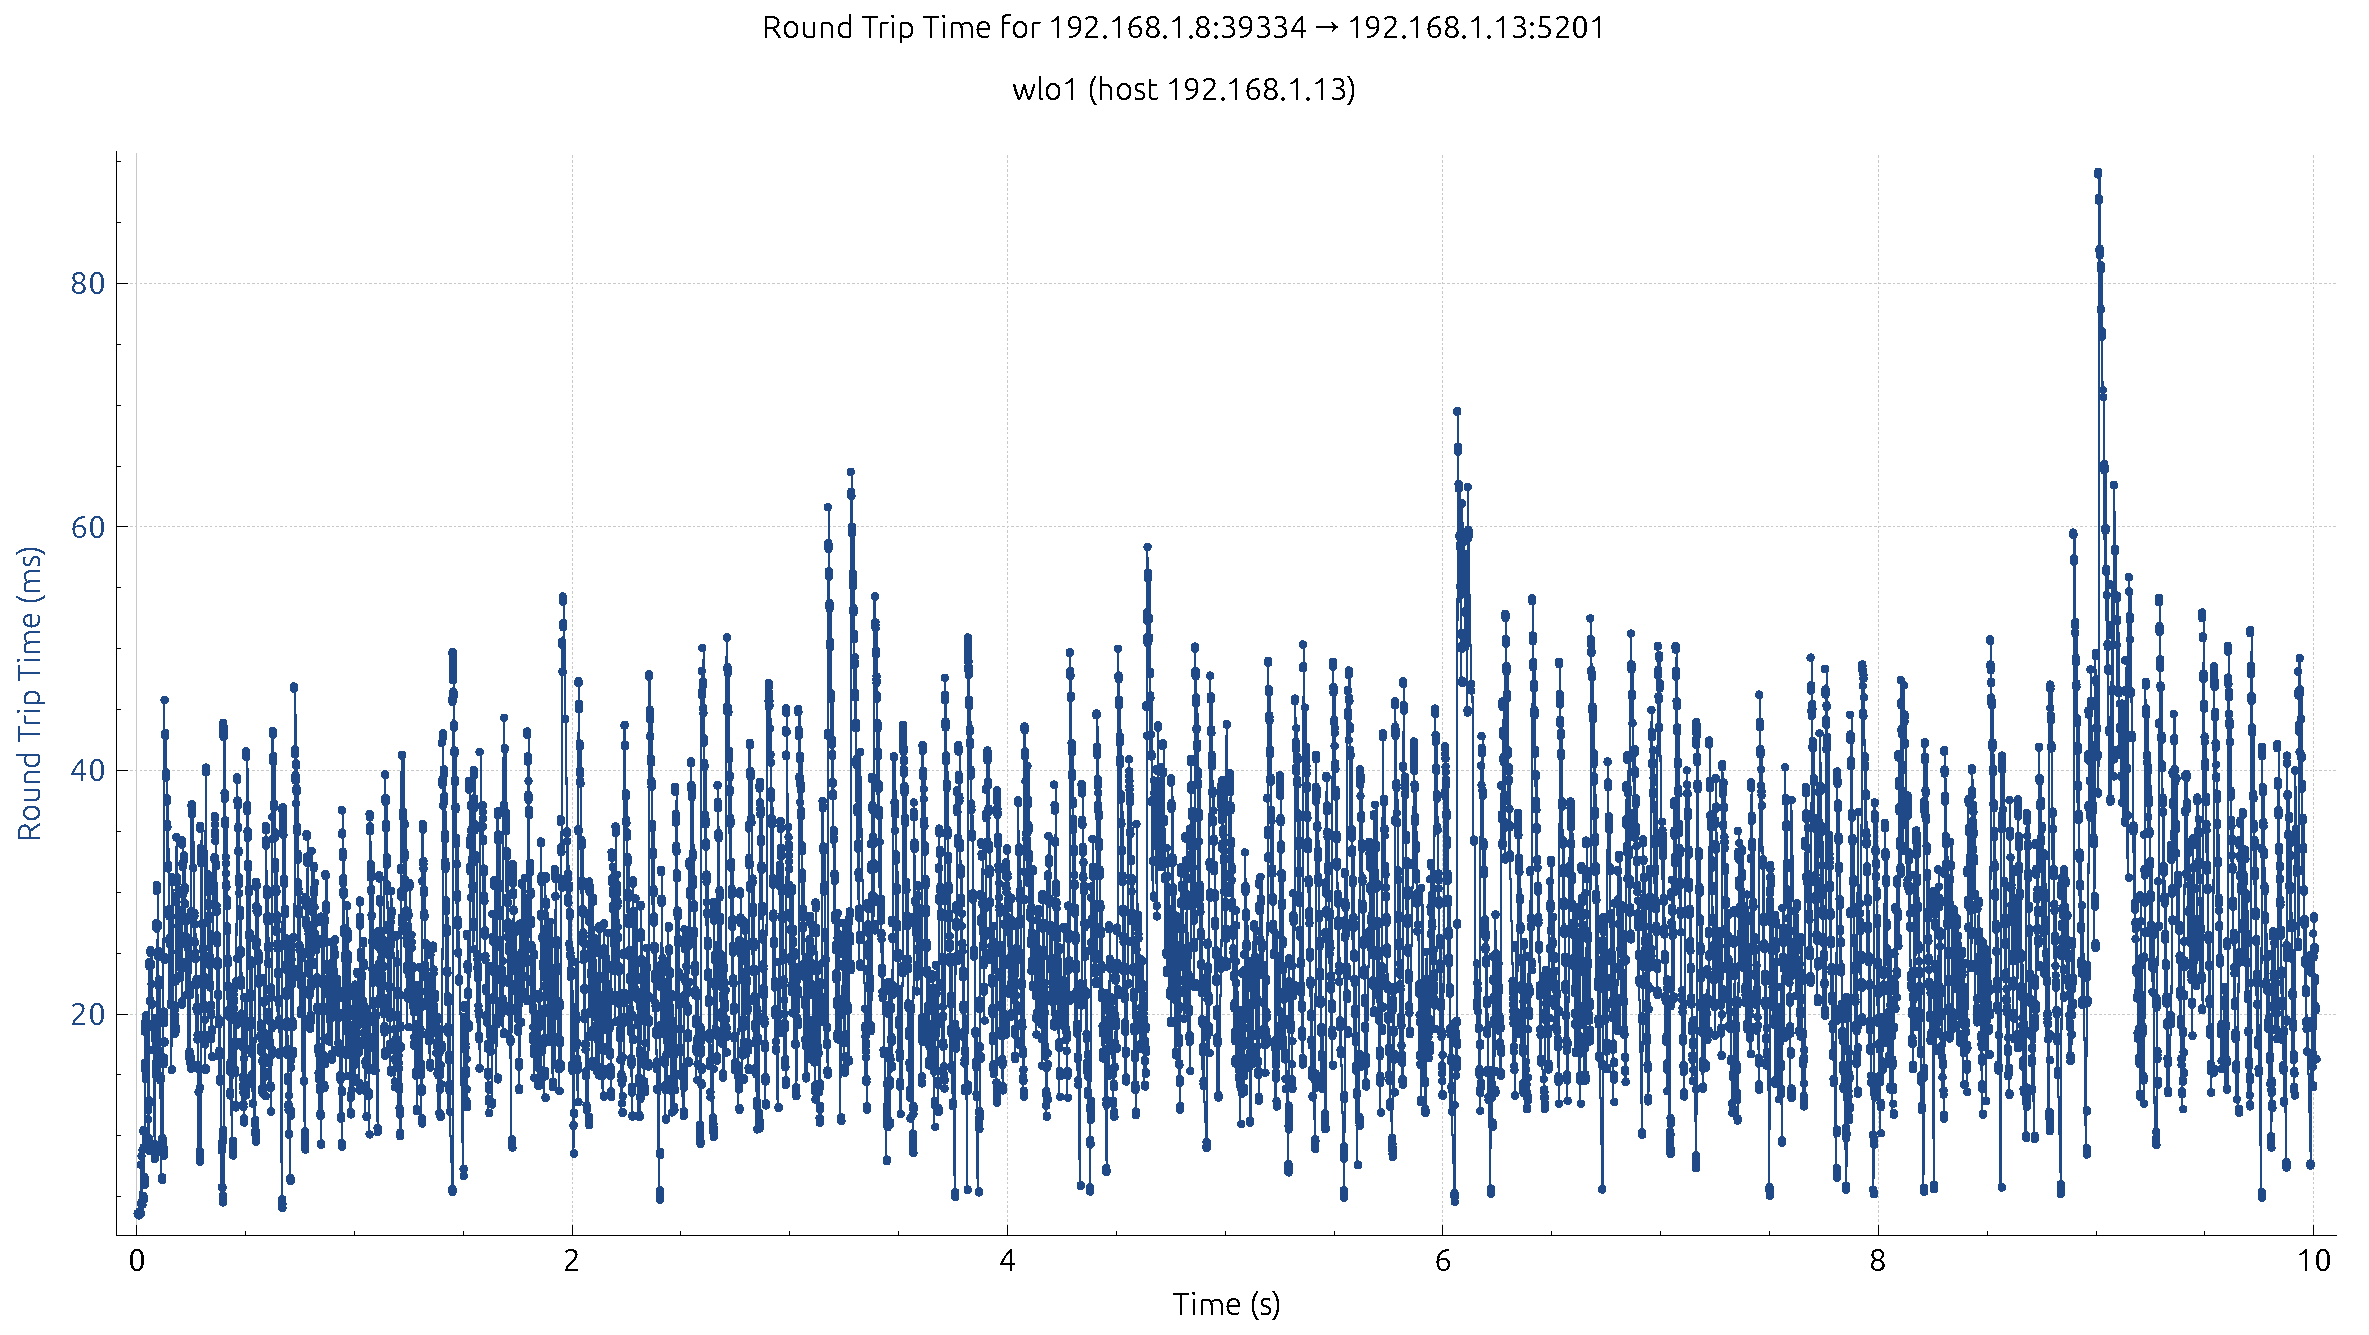
\includegraphics[width=0.9\columnwidth]{images/graphs/RTT/RTT_MIX_MITM_TCP.pdf}
                %     \caption{TCP Round Trip Time in the Shared Capacity Scenario.}
                %     \label{fig:rtt-mitm-tcp}
                % \end{figure}

                The I-O graph for TCP (Fig.~\ref{fig:io-mitm-tcp}) further confirms the impact of the interference. 
                The graph displays irregular intervals and a lower packet transmission rate compared to the mixed scenario without the additional load, demonstrating how the extra traffic disrupts the steady flow of data.

                \begin{figure}[ht]
                    \centering
                    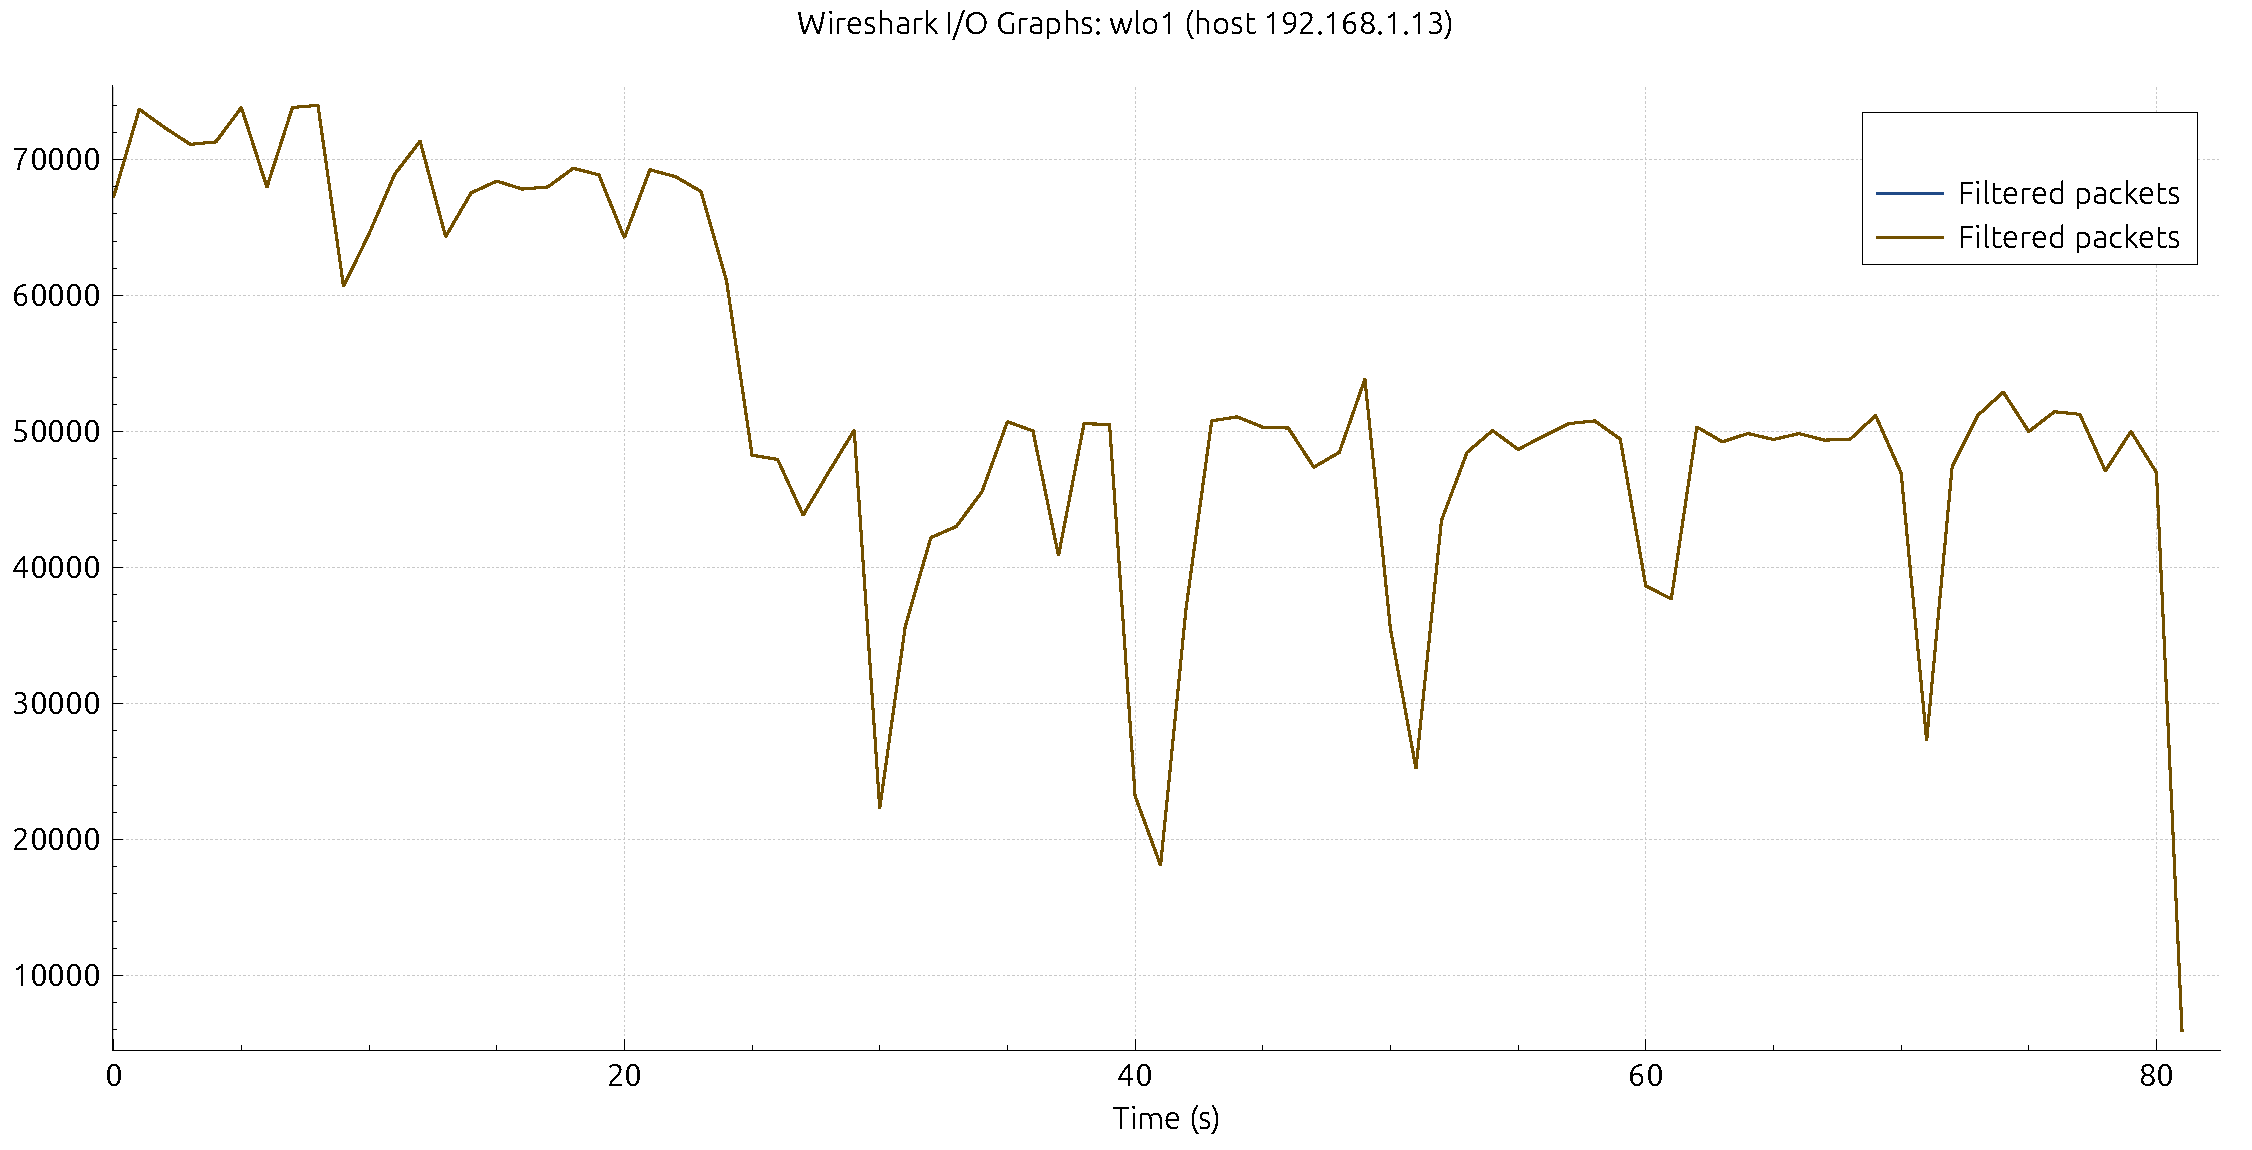
\includegraphics[width=0.9\columnwidth]{images/graphs/I-O/I-O_MIX_MITM_TCP.pdf}
                    \caption{Wireshark I-O Graph for TCP in the Shared Capacity Scenario.}
                    \label{fig:io-mitm-tcp}
                \end{figure}

        \end{enumerate}

    \subsection{UDP Performance} \label{subsec:udp-performance}

        The UDP tests offer an insightful comparison to the TCP results by eliminating congestion control and acknowledgment overhead. The analysis for UDP performance across different scenarios is structured as follows:

        \begin{table}
            \small
            \centering
            \begin{tabular}{|ll|lllll|}
            \hline
            % \multicolumn{2}{|c|}{\multirow{2}{*}{\makecell{\textbf{Test} \\ Client $\rightarrow$ Server}}} & 
            \multicolumn{2}{|c|}{\multirow{2}{*}{\textbf{Test}}} & 
                \multicolumn{5}{c|}{\textbf{UDP: Goodput per flow (Mbps)}} \\
            \cline{3-7}
            \multicolumn{2}{|c|}{} &
                \multicolumn{1}{c|}{Prediction} &
                \multicolumn{1}{c|}{Average} &
                \multicolumn{1}{c|}{Min} &
                \multicolumn{1}{c|}{Max} &
                \multicolumn{1}{c|}{Std} \\
            \hline
            \multicolumn{2}{|c|}{Both WiFi} &
                \multicolumn{1}{c|}{?} &
                \multicolumn{1}{c|}{487.8} &
                \multicolumn{1}{c|}{453.1} &
                \multicolumn{1}{c|}{499.9} &
                \multicolumn{1}{c|}{15.8} \\
            \hline
            \multicolumn{2}{|c|}{Both Ethernet} &
                \multicolumn{1}{c|}{?} &
                \multicolumn{1}{c|}{952.8} &
                \multicolumn{1}{c|}{948.3} &
                \multicolumn{1}{c|}{954.6} &
                \multicolumn{1}{c|}{1.73} \\
            \hline
            \multicolumn{2}{|c|}{Mixed} &
                \multicolumn{1}{c|}{?} &
                \multicolumn{1}{c|}{674.9} &
                \multicolumn{1}{c|}{636.6} &
                \multicolumn{1}{c|}{717.8} &
                \multicolumn{1}{c|}{28} \\
            \hline
            \multicolumn{2}{|c|}{Shared Capacity} &
                \multicolumn{1}{c|}{?} &
                \multicolumn{1}{c|}{472.1} &
                \multicolumn{1}{c|}{355.9} &
                \multicolumn{1}{c|}{699.1} &
                \multicolumn{1}{c|}{121.1} \\
            \hline
            \end{tabular}
            \vspace{0.5cm}
            \caption{UDP Results (Client $\rightarrow$ Server)}
            \label{tab:udp-results}
        \end{table}

        \begin{enumerate}

            \item \textbf{Both Ethernet:} \\
                In the Ethernet configuration, the I-O graph for UDP indicates a steady packet flow, with minimal fluctuations compared to the WiFi scenario.
                
                % \begin{figure}[ht]
                %     \centering
                %     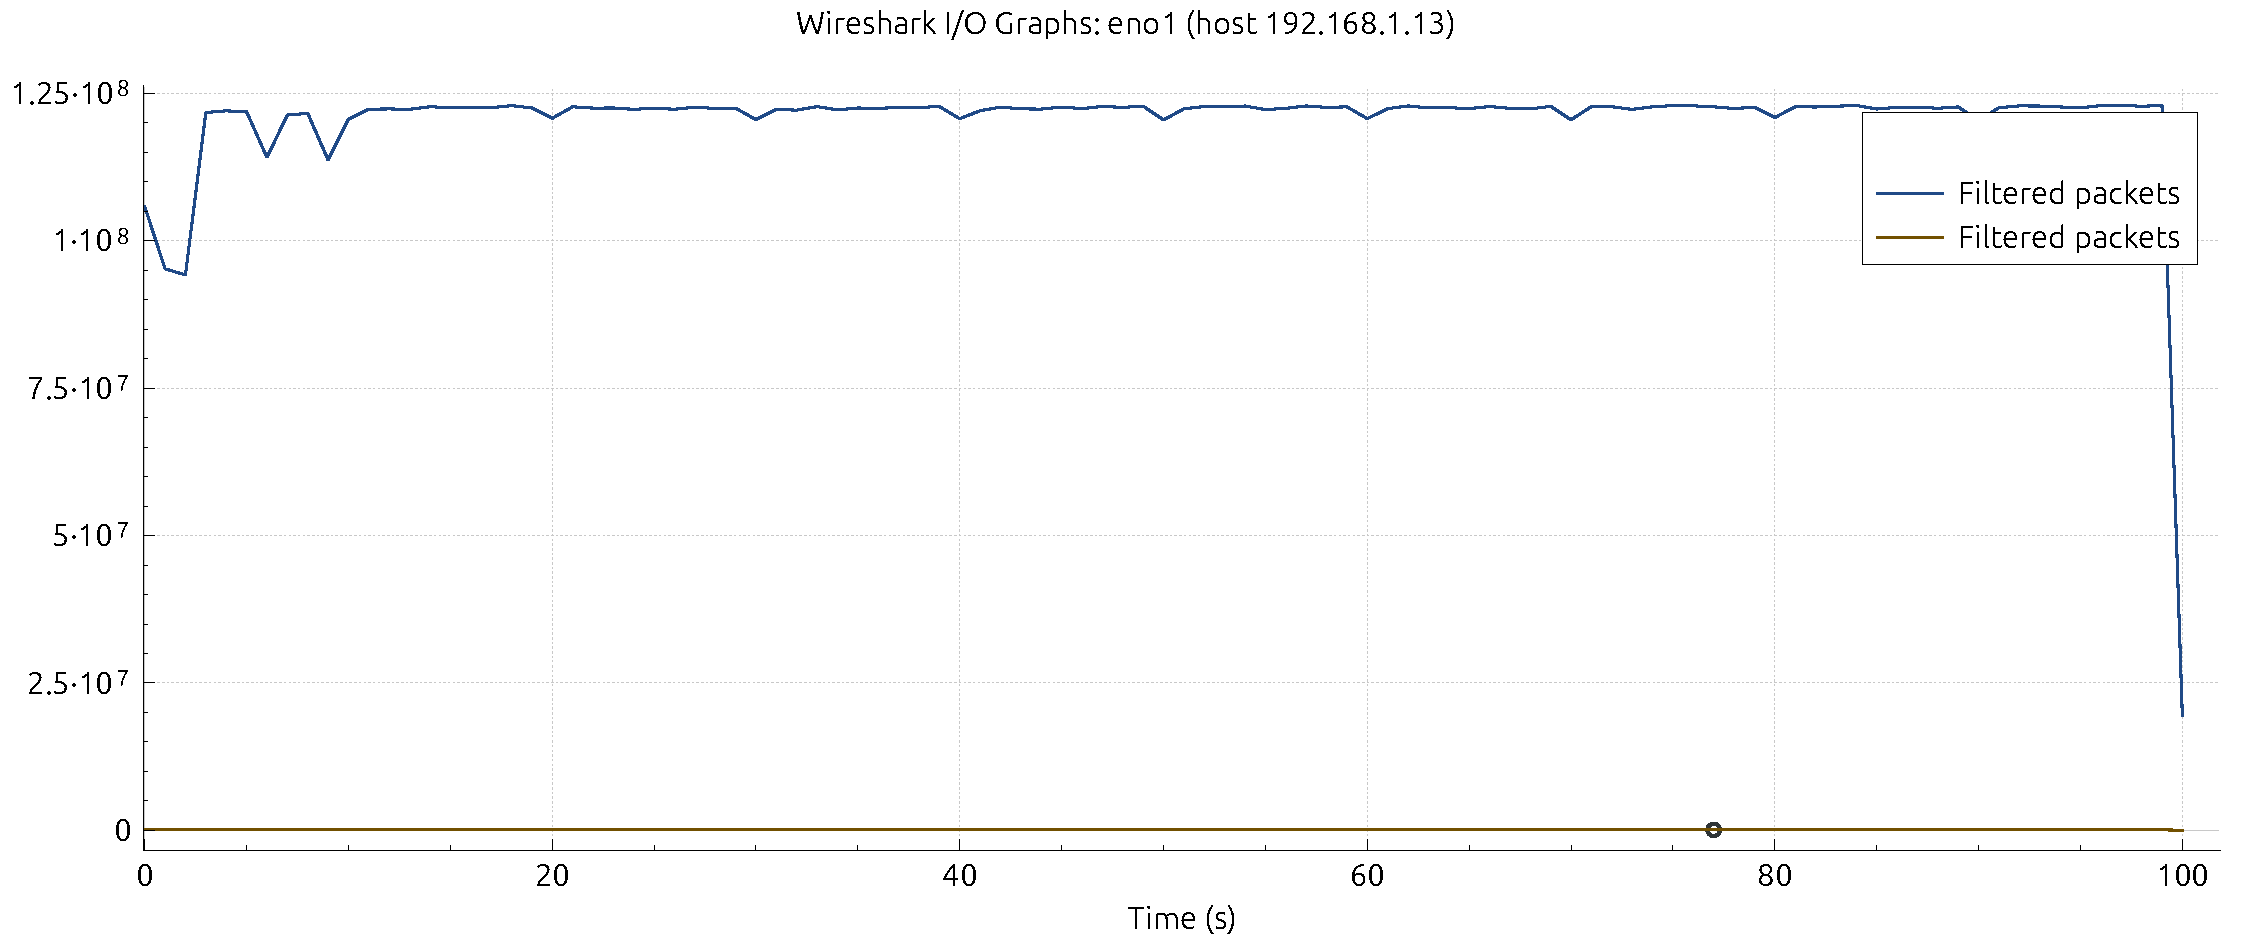
\includegraphics[width=0.9\columnwidth]{images/graphs/I-O/I-O_ETH_UDP.pdf}
                %     \caption{Wireshark I-O Graph for UDP in the Ethernet Scenario.}
                %     \label{fig:io-eth-udp}
                % \end{figure}

                The throughput achieved is very close to the theoretical prediction, confirming that the wired setup reliably supports high-speed data transfer. 
                The absence of retransmission or congestion control overhead in UDP further contributes to this consistent performance.
                
                In summary, the wired (Ethernet) tests demonstrate that both TCP and UDP protocols achieve performance levels very close to their theoretical capacities, with TCP showing stable throughput and low latency, and UDP exhibiting a consistent packet flow and high throughput. 
                This confirms that, in a controlled wired environment, network performance is minimally impacted by protocol overhead or environmental factors.

            \item \textbf{Both WiFi:} \\
                In the WiFi scenario, the I-O graph for UDP demonstrates a more consistent packet flow compared to TCP. 
                However, despite the smoother transmission, the overall throughput remains below the theoretical upper bound. 
                The lack of retransmission mechanisms in UDP allows for slightly higher instantaneous throughput; nonetheless, factors like interference and channel contention continue to impact performance.
                
                % \begin{figure}[ht]
                %     \centering
                %     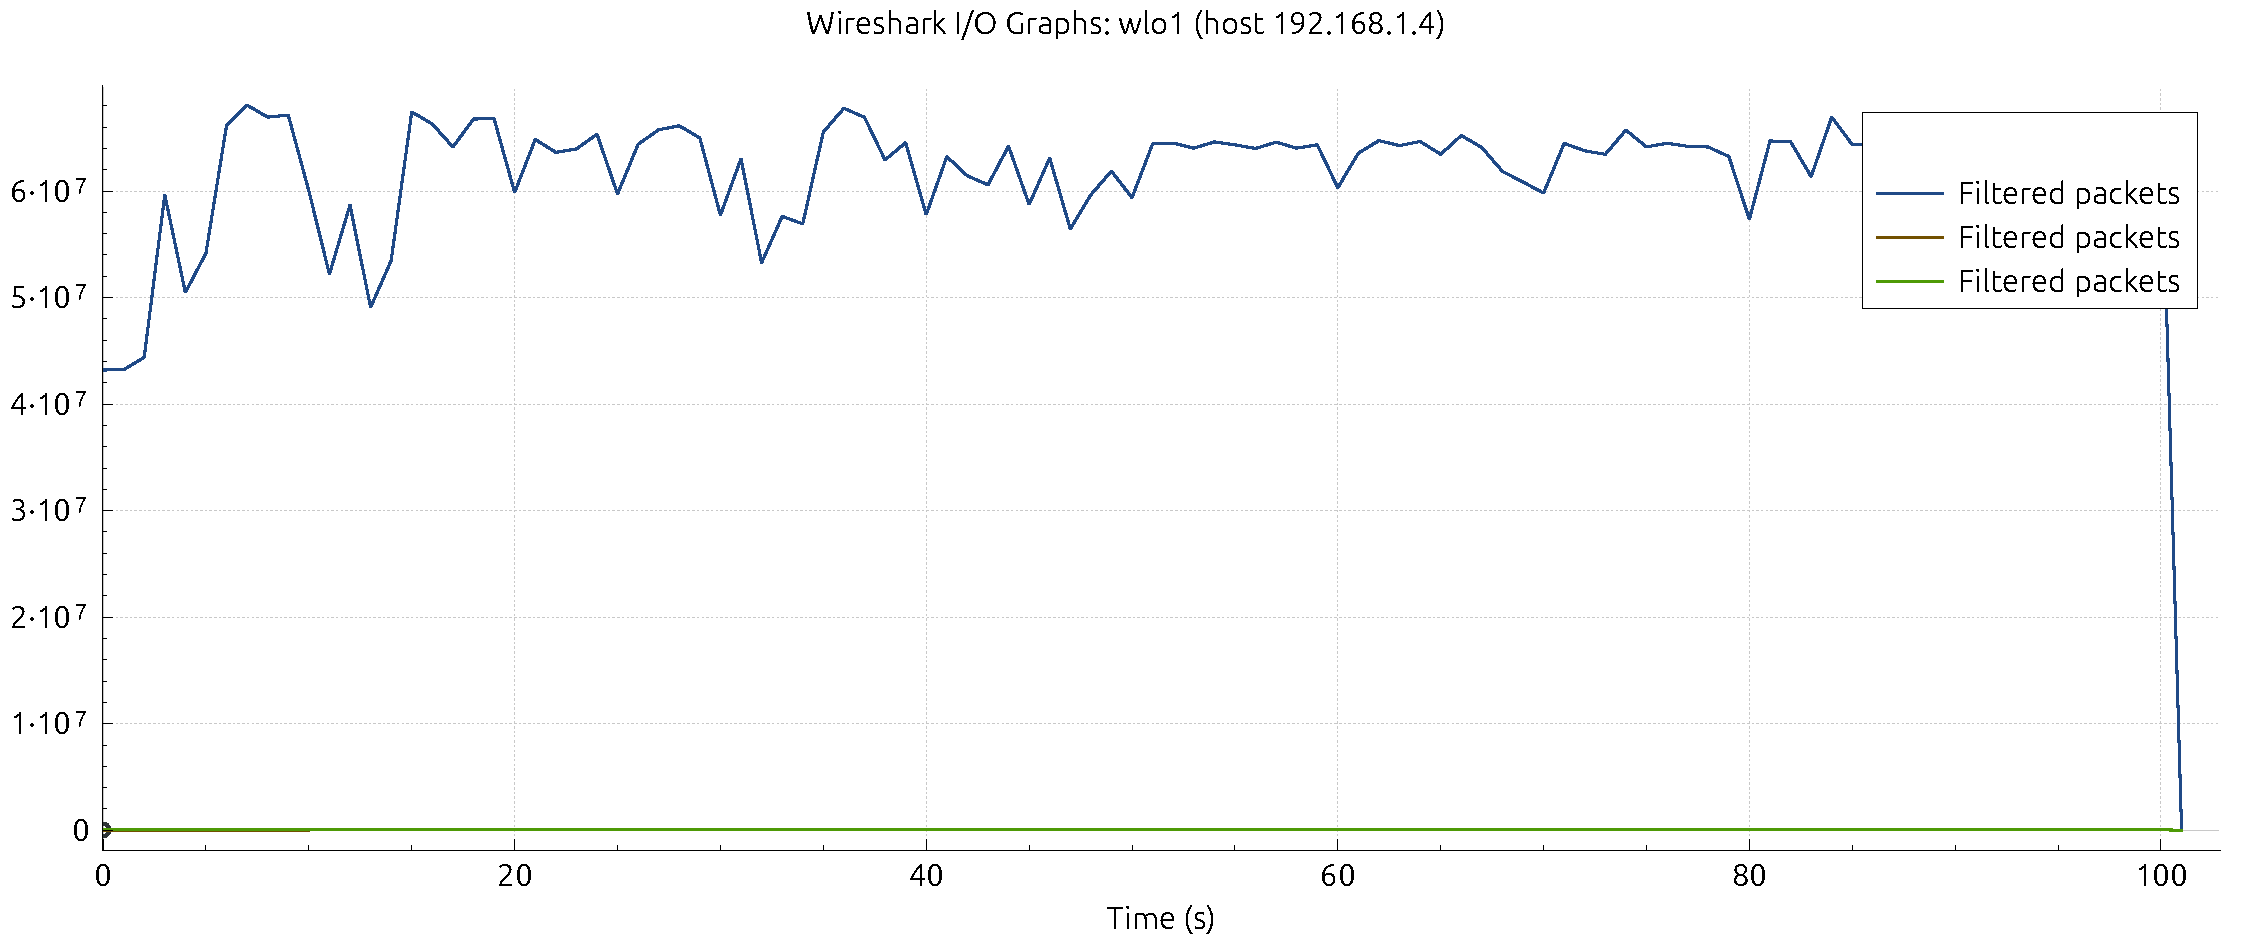
\includegraphics[width=0.9\columnwidth]{images/graphs/I-O/I-O_WiFi_UDP.pdf}
                %     \caption{Wireshark I-O Graph for UDP in the WiFi Scenario.}
                %     \label{fig:io-wifi-udp}
                % \end{figure}

                A direct comparison between TCP and UDP in the WiFi scenario shows that UDP can achieve marginally higher throughput due to its reduced overhead. 
                Nonetheless, both protocols suffer from real-world limitations that prevent them from reaching their theoretical capacities. 
                This discrepancy between capacity and theoretical goodput emphasizes the impact of wireless interference, channel contention, and protocol-specific overhead on performance.

            \item \textbf{Mixed:} \\
                In the mixed scenario, the UDP I-O graph indicates a consistent flow of packets, similar to the TCP case but with slightly less variability due to the absence of congestion control.
                
                % \begin{figure}[ht]
                %     \centering
                %     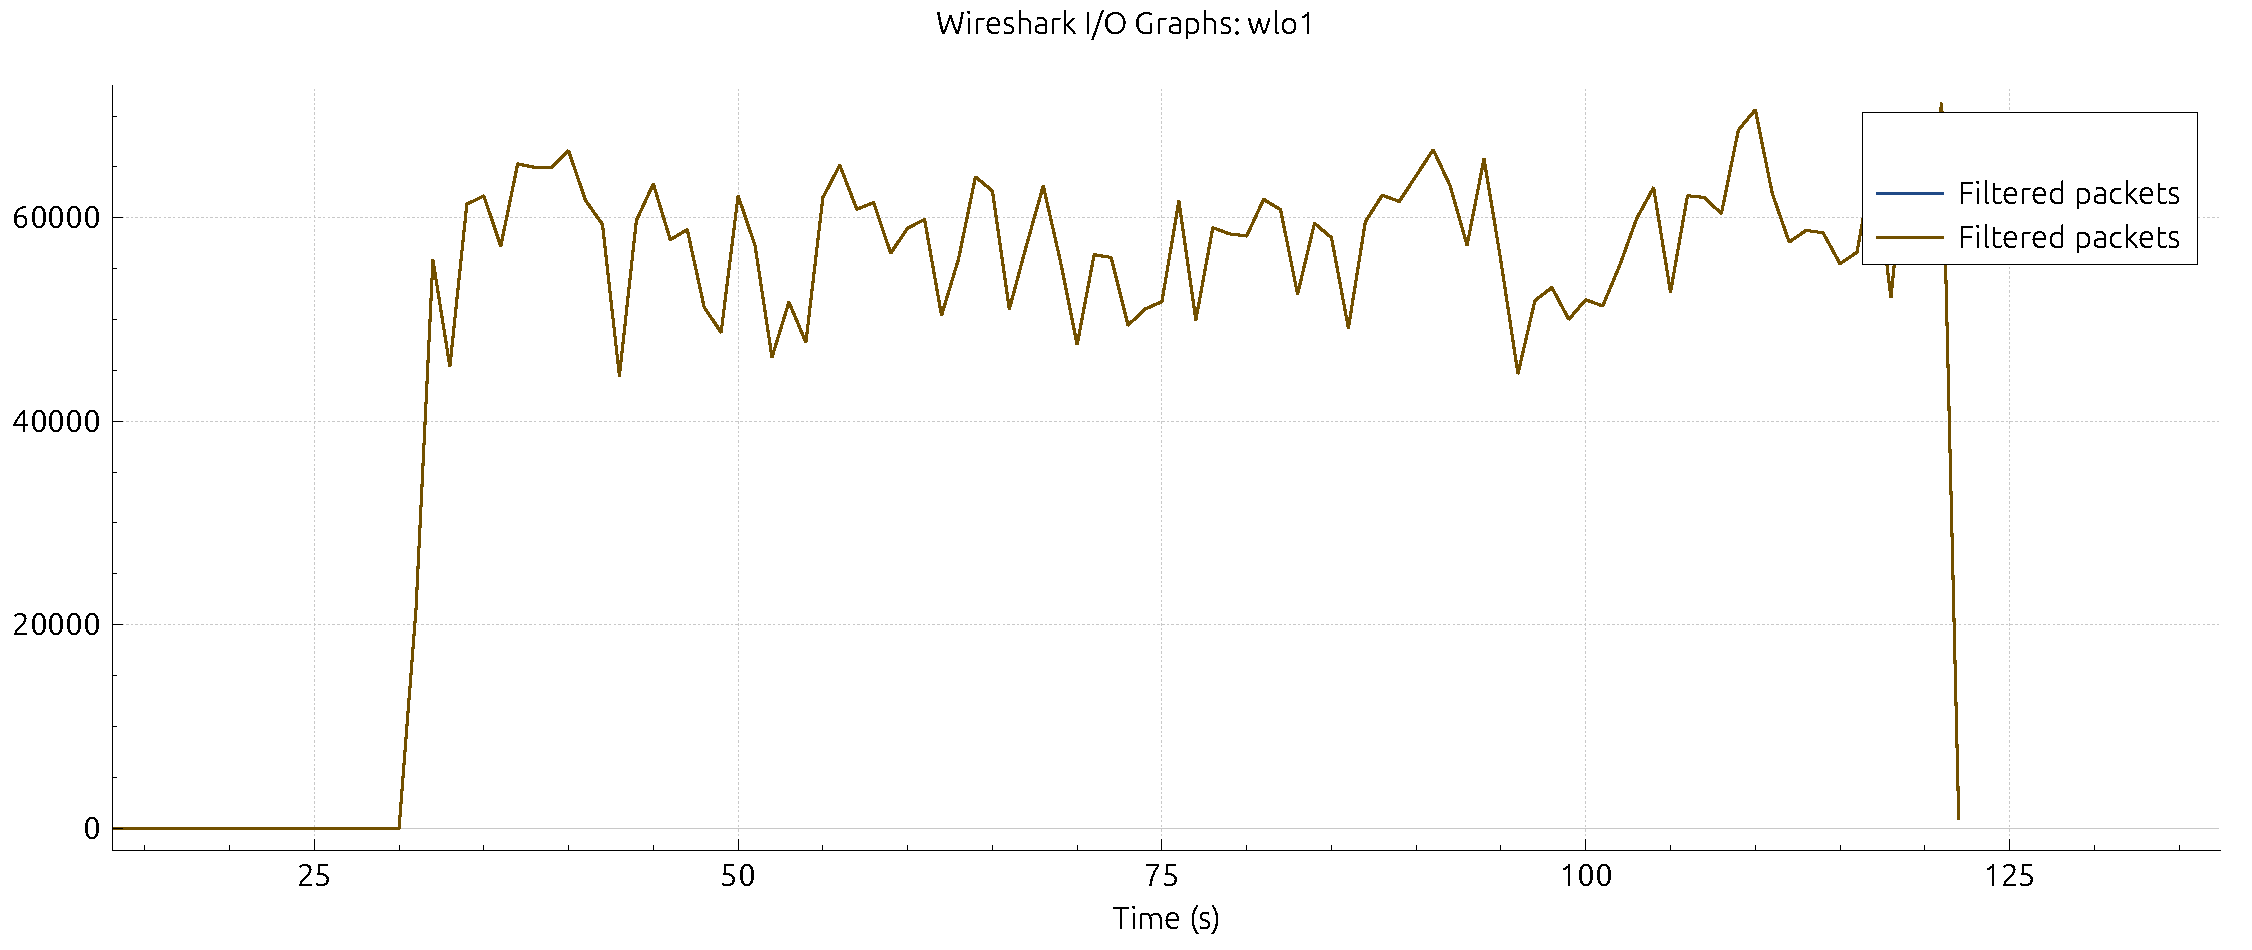
\includegraphics[width=0.9\columnwidth]{images/graphs/I-O/I-O_MIX_UDP.pdf}
                %     \caption{Wireshark I-O Graph for UDP in the Mixed Scenario.}
                %     \label{fig:io-mix-udp}
                % \end{figure}

                The throughput observed is in line with expectations given that only the wireless link acts as the bottleneck. \\

                In summary, the mixed scenario demonstrates that while the presence of a wired connection on one end improves overall latency and stability compared to a full WiFi configuration, the performance remains primarily constrained by the wireless link. 
                Both TCP and UDP protocols achieve throughput values that are consistent with theoretical predictions for a mixed Ethernet/WiFi environment.
                
            \item[3a.] \textbf{Shared Capacity:} \\
                The UDP tests under the shared capacity scenario also reveal the negative impact of the additional download traffic. 
                Although UDP is less affected by protocol overhead, the increased contention for the wireless medium leads to degraded performance.
                The UDP performance in this scenario is indirectly reflected in the I-O graph.
                The steady flow of packets observed in a non-interfered environment is disrupted, resulting in a lower effective throughput.

                % \begin{figure}[ht]
                %     \centering
                %     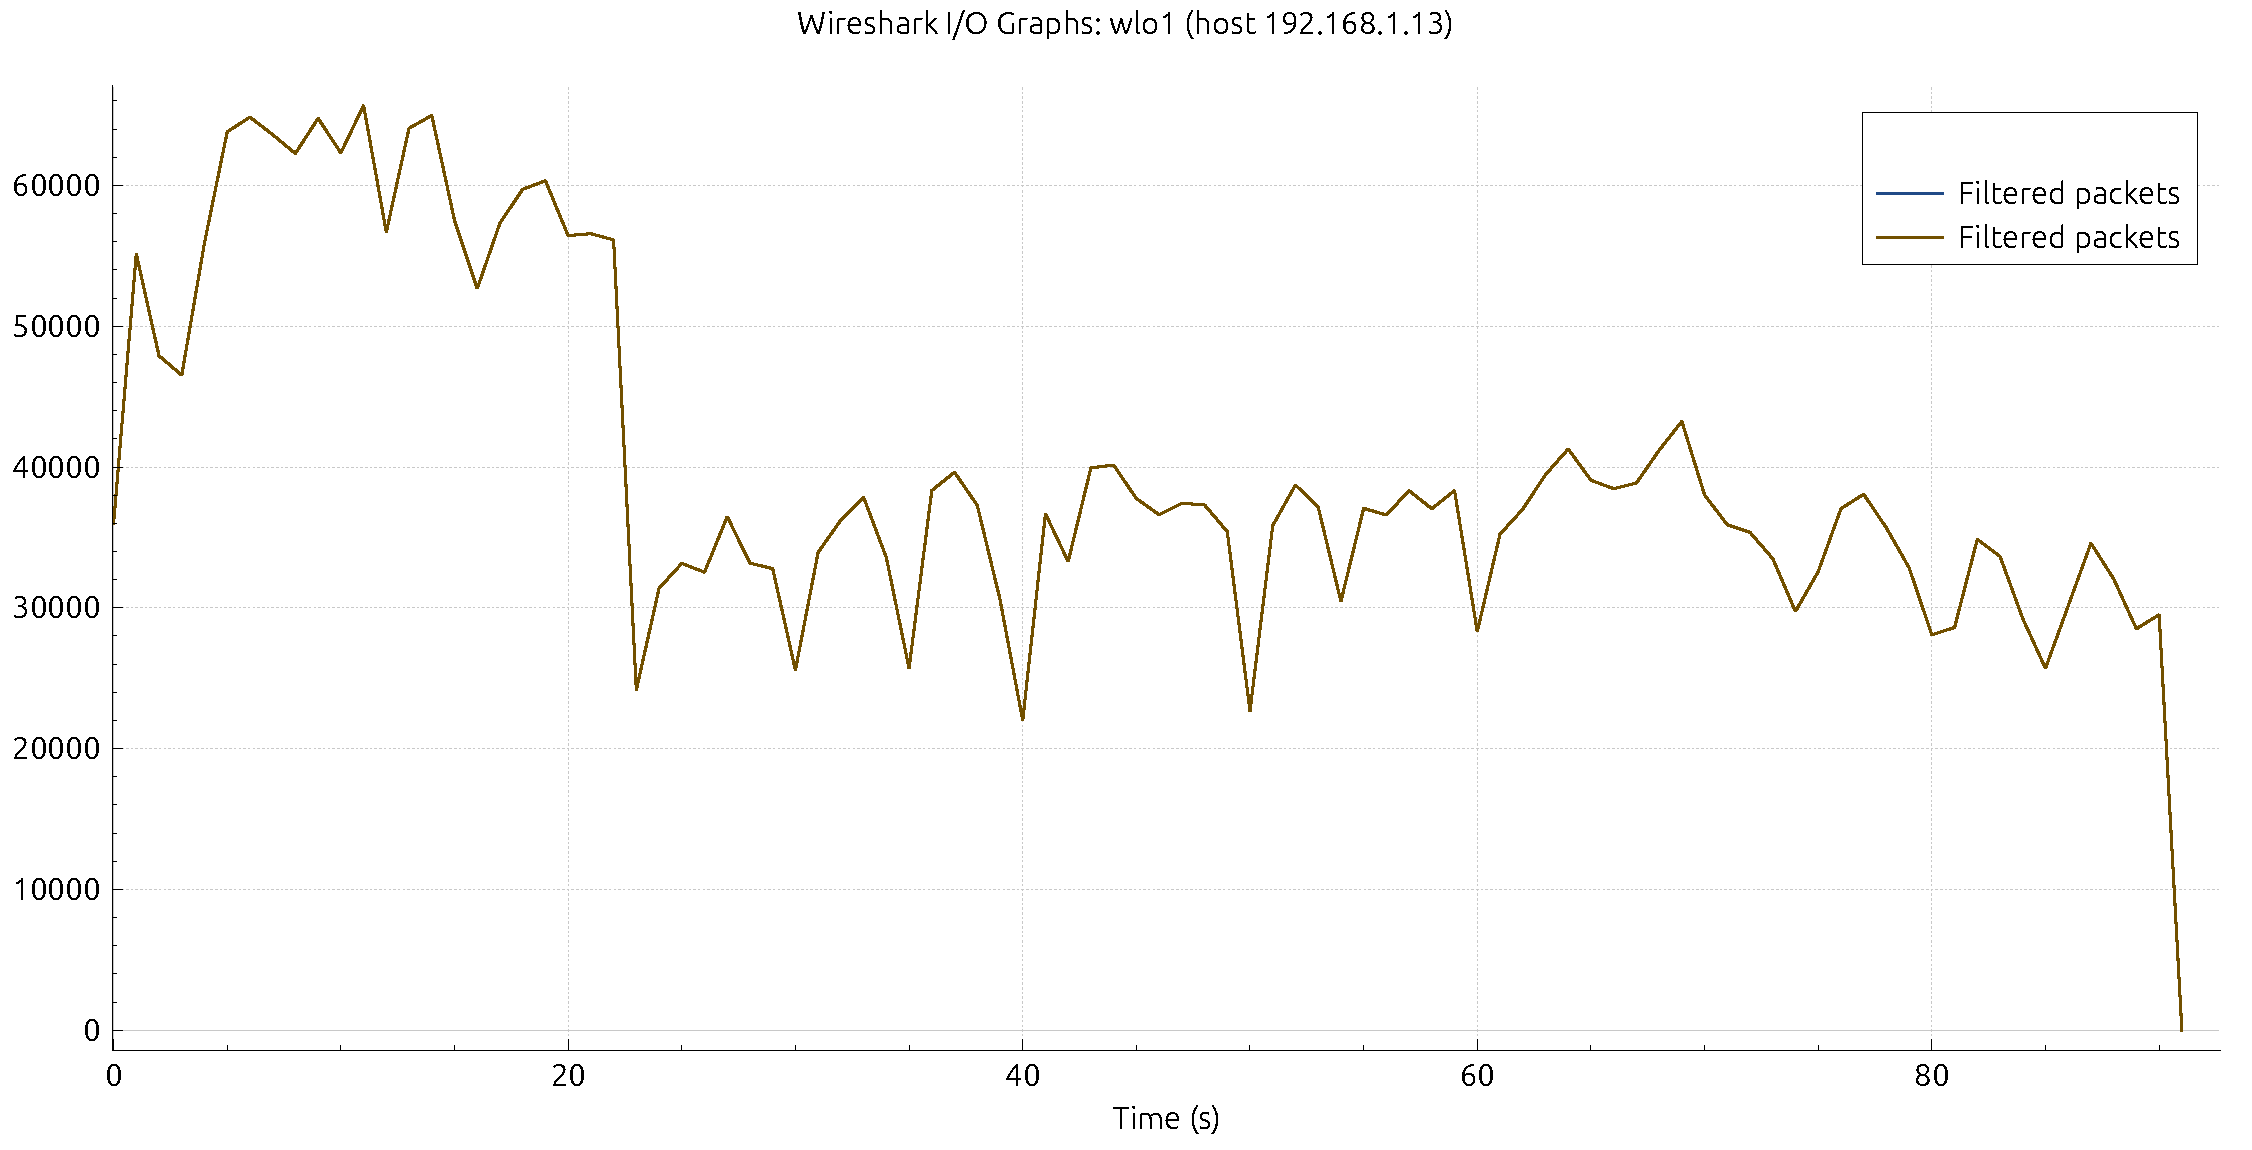
\includegraphics[width=0.9\columnwidth]{images/graphs/I-O/I-O_MIX_MITM_UDP.pdf}
                %     \caption{Wireshark I-O Graph for UDP in the Shared Capacity Scenario.}
                %     \label{fig:io-mitm-udp}
                % \end{figure}

                Despite the inherent resilience of UDP to retransmission delays, the interference from the third host causes a noticeable reduction in performance. 
                The graph shows that the packet flow is not as consistent, further underlining the effects of shared capacity when additional traffic is present.

                Overall, the shared capacity scenario clearly demonstrates that when a third host generates significant traffic (as in the case of streaming a movie), the available network resources are further divided, leading to performance degradation for both TCP and UDP protocols. 
                This scenario highlights the importance of considering real-world usage patterns and interference when designing and evaluating network performance.

        \end{enumerate}
